\documentclass[12pt,twoside,a4paper]{etc/note}
\geometry{left=20mm,right=20mm,top=25mm,bottom=20mm} % задание полей текста
\usepackage{wrapfig}
%% Стиль колонтитулов
% \fancyhead[RO,LE]{\hyperlink{intro}{Содержание}} % Right odd,  Left even
\fancyhead[LO]{\@lecture}        % Right even, Left odd
\fancyhead[R]{}

\fancyfoot[RO,LE]{\thepage}         % Right odd,  Left even
\fancyfoot[RE,LO]{\CourseName}      % Right even, Left odd
\fancyfoot[C]{}
% Un~comment these to erase foot (and comment footrulewidth renewcommand)
%\fancyfoot{}
%\fancyhead[C]{-~\thepage~-}
\renewcommand{\footrulewidth}{0.4pt}
\usepackage{textcomp}

% Новая команда \lecture{№ лекции}{название}
% После этой команды весь текст до следующей такой же команды будет
% принадлежать конкретной лекции, имя которой будет в колонтитуле каждой страницы
\usepackage{xifthen}
\def\@lecture{}%
\newcommand{\lecture}[2]{
    \ifthenelse{\isempty{#2}}{%
        \def\@lecture{Лекция #1}%
    }{%
        \def\@lecture{Лекция #1: #2}%
    }%
    \section{\@lecture}
}

\def\@lecture{}%
\newcommand{\question}[2]{
    \ifthenelse{\isempty{#2}}{%
        \def\@lecture{Билет #1}%
    }{%
        \def\@lecture{Билет #1: #2}%
    }%
    \section{\@lecture}
}
% ------------ Text settings ------------
%%% Гиппер ссылки
\renewcommand{\linkcolor}{blue}
\renewcommand{\citecolor}{green}
\renewcommand{\filecolor}{magenta}
\renewcommand{\urlcolor}{NavyBlue}

\usepackage{multicol}	   % Для текста в нескольких колонках

% -----------  Images -----------
\graphicspath{{images/}{img/}{figures/}{fig/}}  % Путь к папкам с картинками
\newcommand{\figL}[3]{%      Для быстрой вставки картинок
    \begin{figure}[h!]
        \centering
        \includegraphics[width=#2\textwidth]{#1}
        \label{fig:#3}
    \end{figure}%
}
\newcommand{\fig}[2]{%    
    \begin{figure}[h!]
        \centering
        \includegraphics[width=#2\textwidth]{#1}
    \end{figure}%
}

% ----------- Math short-cats
\newcommand{\R}{\ensuremath{\mathbb{R}}}
\newcommand{\N}{\ensuremath{\mathbb{N}}}
\newcommand{\Cx}{\ensuremath{\mathbb{C}}}
\newcommand{\Z}{\ensuremath{\mathbb{Z}}}
\newcommand{\E}{\ensuremath{\mathbb{E}}}
\newcommand{\Q}{\ensuremath{\mathbb{Q}}}
\def\CB{\mathcal{B}}
\def\CC{\mathcal{C}}
\def\CE{\mathcal{E}}
\def\CR{\mathcal{R}}
\def\CA{\mathcal{A}}
% \def\CF{\mathcal{F}}
\def\CG{\mathcal{G}}
\def\CS{\mathcal{S}}
\def\CD{\mathcal{D}}
\def\CH{\mathcal{H}}
\def\CP{\mathcal{P}}
\def\CM{\mathcal{M}}
\def\FB{\mathfrak{B}}

% You can write your commands below
\usepackage{gensymb}
\usepackage{enumitem}
\usepackage{amsmath}
\newcommand{\F}{\ensuremath{\mathcal{F} }}
\newcommand{\Anu}{\ensuremath{\mathcal{A}_{\nu}}}
\DeclareMathOperator{\FDU}{FDU}

% ----------- Math and theorems -----------
\usepackage[many]{tcolorbox}
\usepackage{mdframed}
\usepackage[dvipsnames]{xcolor}

\newtheorem*{remark}      {Замечание}
\newtheorem*{next0}      {Следствие}
\newtheorem*{next1}      {Следствие 1}
\newtheorem*{next2}      {Следствие 2}
\theoremstyle{definition}
\newtheorem{lemma}{Лемма}[section]
\newtheorem{claim}[lemma]{Утверждение}
\newtheorem{theorem_}[lemma]{Теорема}
\newenvironment{theorem}%
{\begin{mdframed}[backgroundcolor=black!30!white!30]
        % \setlength{\topsep}{-\parskip}\setlength{\partopsep}{0pt}
        \begin{theorem_}}%
            {\end{theorem_}\end{mdframed}}

\theoremstyle{definition}
\newtheorem{definition}[lemma]{Определение}
\tcolorboxenvironment{definition}{
    enhanced,
    borderline={0.8pt}{0pt}{gray!70},
    borderline={0.4pt}{2pt}{black},
    boxrule=0.4pt,
    colback=pink!70!white!30,
    coltitle=black,
    sharp corners
}
\usepackage{ulem}
\newcommand{\mdef}[1]
{\! \textit{\uwave{\textcolor{red!10!black}{#1}}}}
% http://dkhramov.dp.ua/Comp.LatexCyrillicFonts#.XMrWLegzaUk


%https://tex.stackexchange.com/questions/223694/how-to-draw-a-text-box-with-shadow-borders-in-latex

\newtheorem{exercise_}[lemma]{Пример}
\newenvironment{exercise}%
{\begin{tcolorbox}[enhanced,width=\textwidth,center upper,drop fuzzy shadow southwest,
            colframe=red!50!black,colback=orange!100!yellow!50!white!30]
        \begin{exercise_}}%
            {\end{exercise_}\end{tcolorbox}}

\usepackage{dashrule}
\renewenvironment{proof}{\smallskip{\noindent\Large
        \color{red!50!black}\itshape$\lhd$ \normalsize Начало доказательства
        \hdashrule[0.5ex]{0.65\textwidth}{0.5mm}{3mm 3pt 1mm 2pt} }
    \small\itshape}{{\color{red!50!black}
            \hdashrule[0.5ex]{0.66\textwidth}{0.5mm}{3mm 3pt 1mm 2pt}
            \normalsize Конец доказательства \Large$\rhd$}}

\newenvironment{solution}{\smallskip{\noindent\Large
        \color{red!50!black}\itshape$\lhd$ \normalsize Начало решения
        \hdashrule[0.5ex]{0.75\textwidth}{0.5mm}{3mm 3pt 1mm 2pt} }
    \small}{{\color{red!50!black}
            \hdashrule[0.5ex]{0.75\textwidth}{0.5mm}{3mm 3pt 1mm 2pt}
            \normalsize\itshape Конец решения \Large$\rhd$}}

% Обводка кружочком множеств
\usepackage{tikz}
\usetikzlibrary{decorations.pathreplacing,shapes.misc,patterns}
\newcommand*\circled[1]{\tikz[baseline=(char.base)]{
        \node[shape=circle,draw,inner sep=2pt] (char) {#1};}}

\counterwithin*{equation}{section}

\usepackage{stackrel}
\newsavebox\MBox
\newcommand\Cline[2][red]{{\sbox\MBox{$#2$}%
            \rlap{\usebox\MBox}\color{#1}\rule[-1.2\dp\MBox]{\wd\MBox}{0.5pt}}}

%%% Почти всю шаблонную информацию можно менять тут
\newcommand{\CourseDate}{\the\year{}}
\newcommand{\CourseName}{Мера Лебега}
\renewcommand{\FullCourseNameFirstPart}{\so{МЕРА}}
\renewcommand{\FullCourseNameSecondPart}{\so{И~ИНТЕГРАЛ~ЛЕБЕГА}}
\renewcommand{\SemesterNumber}{IV СЕМЕСТР}
\renewcommand{\SchoolName}{Физтех-школа: \textit{ФПМИ}}
\renewcommand{\TrackName}{Направления: \textit{ПМФ}}
\renewcommand{\LecturerInitials}{Лектор: \textit{Гусев Николай Анатольевич}\\ngusev@phystech.edu}
% You can add up to 4 authors (AuthorA, AuthorB, AuthorC, ...)
\renewcommand{\AuthorA}
    {\href{https://vk.com/s0mth1ng}{\textit{Максим Иванов}}}
%\renewcommand{\AuthorB}
%    {\href{https://vk.com/}{\textit{Фамилия2 Имя2}}}
% You can leave \OverleafLink or \OverleafLink empty to make them disappear from the title page, or not empty to make them appear automatically
\renewcommand{\OverleafLink}{}
% \renewcommand{\GithubLink}{https://github.com/MIPT-Group/Lectures_Tex_Club}
\renewcommand{\ImageName}{logo_LTC}

\begin{document}
\maketitle
\newpage

\tableofcontents
\setcounter{section}{10}
\section{Глава 11. Ряды Фурье.}
\subsection{Коэффициенты Фурье.}
Рассматриваем функции, суммируемые с квадратом на промежутке $I\subset \R$ --- это измеримые на $I$ функции, такие что $f^2\in L(I)$, где $L(I)$ --- множество суммируемых на $I$ функций.

\begin{prop}
	Множество суммируемых с квадратом на $I$ функций образуют линейное пространство, причем произведение любых двух таких функций суммируемо на $L(I)$.
\end{prop}

\begin{proof}
	Пусть $f_1, f_2$ суммируемы с квадратом, тогда $|f_1(x)\cdot f_2(x)|\leqslant\dfrac{1}{2} \left({f_1}^2(x)+{f_2}^2(x)\right)$. Произведение измеримых функций является измеримой функцией, это произведение по модулю не превосходит суммируемой функции, тогда по признаку суммируемости, это произведение является измеримой функцией. Для доказательства линейности пространства, докажем, что $f_1(x)+f_2(x)$ тоже суммируема с квадратом. Сумма измеримых функций --- измерима. $(f_1(x)+f_2(x))^2={f_1}^2(x)+2\cdot f_1(x)\cdot f_2(x) + {f_2}^2(x)$ --- каждое слагаемое суммируемое, значит и все выражение суммируемо.
\end{proof}

Попытаемся ввести скалярное произведение двух функций, как $$<f_1, f_2>=\int\limits_{I}f_1(x)\cdot f_2(x)d\mu(x).$$ При проверке свойств скалярного произведения, получим, что свойство $<f,f>=0\Leftrightarrow f=0$ не выполняется, так как $<f,f>=0\Leftrightarrow \int\limits_{I}f^2(x)\cdot d\mu(x)\Leftrightarrow f=0$ почти всюду. Поэтому необходимо ввести отношение эквивалентности и отождествить функции которые совпадают почти всюду.

\begin{Def}
	$L_2(I)$ --- множество суммируемых с квадратом функций, с отождествлением эквивалентных (то есть совпадающих почти всюду на $I$) функций. Причем, оно является евклидовым пространством.
\end{Def}

Теперь, к примеру, функции Дирихле или Римана не отличимы от тождественного нуля.
\begin{prop}[Неравенство Коши-Буняковского-Шварца]\ \\
	$|<f_1,f_2>|^2\leqslant <f_1,f_1>\cdot<f_2,f_2>$
	
	$\left(\int\limits_{I}f_1(x)\cdot f_2(x)d\mu(x)\right)^2\leqslant\int\limits_{I}{f_1}^2(x)d\mu(x)\cdot \int\limits_{I}{f_2}^2(x)d\mu(x)$.
\end{prop}

\begin{Def}
	Ортогональная система функций из $L_2(I)$ --- это последовательность $\{e_n(x)\}_{n=1}^\infty$ ненулевых элементов $L_2(I)$, такая что $<e_n,e_m>=0, n\ne m$. Если при этом $<e_n,e_n>=1, n=1,\ldots$, то $\{e_n(x)\}_{n=1}^\infty$ называется ортонормированной системой.
\end{Def}

\begin{linkex}{https://youtu.be/yxBOm0XzFnQ?t=1134}[ортогональных систем]\ 
	\begin{enumerate}
		\item $I=[-1,1]$ Многочлены Лежандра $P_n(x)=\dfrac{1}{n!\cdot2^n}\dfrac{d^n}{dx^n}\left((x^2-1)^n\right), P_0(x)=1$.
		\begin{proof}(Первый вариант доказательства)
			Необходимо проверить, что при $n>k\geqslant 0 \Rightarrow <P_n, P_k>=0$. 
			\begin{multline*}
				\int\limits_{-1}^1\dfrac{d^n}{dx^n}\left((x^2-1)^n\right)\dfrac{d^k}{dx^k}\left((x^2-1)^k\right)dx=[\text{интегрируем по частям}]=\\=\underbrace{\dfrac{d^{n-1}}{dx^{n-1}}((x^2-1)^n)\dfrac{d^k}{dx^k}((x^2-1)^k)|_{-1}^1}_{=0, \text{см. дальше}}-\int\limits_{-1}^1\dfrac{d^{n-1}}{dx^{n-1}}((x^2-1)^n)\dfrac{d^{k+1}}{dx^{k+1}}((x^2-1)^k)dx.
			\end{multline*}
			Заметим, что $(x^2-1)^n$ --- представляет собой многочлен степени $2n$. Раскладывая многочлен по формуле Тейлора с центром в единице, получим конструкцию $(x-1)^n\cdot(\ldots)$. А значит все производные от $(x^2-1)^n$ в единичке, вплоть до $n-1$ порядка, равны нуля. Аналогично в $-1$. Продолжая интегрирование по частям получим: $$(-1)^n\int\limits_{-1}^1(x^2-1)^n\dfrac{d^{n+k}}{dx^{n+k}}((x^2-1)^k)dx.$$
			Так как $n>k$, то $n+k>2k$ и производная $n+k$ степени от $(x^2-1)^k$ равна тождественному нулю.
		\end{proof}
		\begin{proof}(Второй вариант доказательства)
			Необходимо проверить, что при $n>k\geqslant 0 \Rightarrow <P_n, P_k>=0 \\
			\mathcal{J}=\int\limits_{-1}^1\dfrac{d^n}{dx^n}\left((x^2-1)^n\right)\dfrac{d^k}{dx^k}\left((x^2-1)^k\right)dx=0$.
			
			Введем вспомогательное утверждение: $\dfrac{d^j}{dx^j}((x^2-1)^n)=(x-1)^{n-j}g_j(x)$, где $g_j(x)$ --- многочлены степени $n$, для $j=0,1,\ldots, n$. Доказательство по индукции. 
			
			При $j=0$ никаких производных не берем, $g_0(x)=(x+1)^n$. 
			
			$\dfrac{d^{j+1}}{dx^{j+1}}((x^2-1)^n)=\left((x-1)^{n-j}g_j(x)\right)'=(n-j)(x-1)^{n-j-1}g_j(x)+(x-1)^{n-j}g_j'(x)=(x-1)^{n-(j+1)}((n-j)g_j(x)+(x-1)g_j'(x))$. В качестве $g_{j+1}(x)=(n-j)g_j(x)+(x-1)g_j'(x)$.
			
			Следующее утверждение будет также справедливо: $\dfrac{d^j}{dx^j}((x^2-1)^n)=(x+1)^{n-j}g_j(x)$, где $g_j(x)$ --- многочлены степени $n$, для $j=0,1,\ldots, n$.
			
			Возвращаясь к доказательству получаем, что
			
			$\dfrac{d^{j}}{dx^j}((x^2-1)^n)|_{x=\pm1}=0, j=0,\ldots,n-1$. Интегрируя по частям $\mathcal{J}$, загоняя первый сомножитель под дифференциал, получаем: 
			\begin{multline*}
				\mathcal{J}=-\int\limits_{-1}^1\dfrac{d^{n-1}}{dx^{n-1}}((x^2-1)^n)\dfrac{d^{k+1}}{dx^{k+1}}((x^2-1)^k)dx=\overset{n \text{ раз интегрируя по частям}}{\ldots}=\\=(-1)^n\int\limits_{-1}^1(x^2-1)^n\dfrac{d^{k+1}}{dx^{k+n}}((x^2-1)^k)dx=0,
			\end{multline*}
			так как берем производную порядка больше чем степень многочлена:$k+n>2\cdot  k$.
		\end{proof}
		\item Стандартная тригонометрическая система. $I=[a,a+2\pi]$. Система функций: $\dfrac{1}{2}, cos(x),sin(x),cos(2x),sin(2x),\ldots$.
		\begin{proof}
			Необходимо проверить пять типов равенств:
			
			$\int\limits_{I}\cos(nx)\cos(mx)dx=0, m\ne n.$
			
			$\int\limits_{I}\sin(nx)\sin(mx)dx=0, m\ne n.$
			
			$\int\limits_{I}\cos(nx)\sin(mx)dx=0.$
			
			$\int\limits_{I}\frac{1}{2}\cos(nx)dx=0.$
			
			$\int\limits_{I}\frac{1}{2}\sin(nx)dx=0.$
			
			Проверим
			\begin{multline*}
				\int\limits_{-\pi}^{\pi}\cos(nx)\cos(mx)dx=\frac{1}{2}\int\limits_{-\pi}^{\pi}(\cos((m+n)x)+\cos((m-n)x))dx=\\= \frac{1}{2(m+n)}\sin((m+n)x)|_{-\pi}^{\pi}+\frac{1}{2(m-n)}\sin((m-n)x)|_{-\pi}^{\pi}=0, m\ne n
			\end{multline*} 
		\end{proof}
	\end{enumerate}
\end{linkex}

\begin{Def}
	Если $\{e_n(x)\}_{n=1}^\infty$ --- ортогональная система в $L_2(I)$, то $\forall f\in L_2(I)$ коэффициентами Фурье называются числа $\alpha_n=\dfrac{<f,e_n>}{<e_n,e_n>}$. Функциональный ряд $\sum\limits_{n=1}^\infty\alpha_n e_n(x)$ называется рядом Фурье функции $f$ по системе $\{e_n(x)\}_{n=1}^\infty$.
\end{Def}

Рассмотрим ряды Фурье в стандартной тригонометрической системе: 
$$\begin{aligned}
	a_n&=\dfrac{\int\limits_I f(x)\cos nx d\mu(x)}{\int\limits_I \cos^2nxdx}=\dfrac{1}{\pi}\int\limits_{[-\pi,\pi]}f(x)\cos nx d\mu(x), n=1,2,\ldots\\
	a_0&=\dfrac{\int\limits_I \dfrac{1}{2}f(x) d\mu(x)}{\int\limits_I {\left(\dfrac{1}{2}\right)}^2dx}=\dfrac{1}{\pi}\int\limits_{[-\pi,\pi]}f(x) d\mu(x)\\
	b_n&=\dfrac{\int\limits_{I}f(x)\sin nx d\mu(x)}{\int\limits_{I}\sin^2nxdx}=\dfrac{1}{\pi}\int\limits_{[-\pi,\pi]}f(x)\sin nxd\mu(x), n=1,2,\ldots
\end{aligned}
\eqno(1)
$$
\label{form_1_2}
Тригонометрический ряд Фурье:
$$f(x)\sim \dfrac{a_0}{2}+\sum\limits_{n=1}^\infty(a_n\cos nx+b_n\sin nx)
\eqno(2)
$$

Предположение о том что $f\in L_2$ в тригонометрической системы излишнее, достаточно предполагать, что
$f\in L_1[-\pi,\pi]$, где $L_1[-\pi,\pi]$ --- линейное нормированное пространство, состоящее из классов эквивалентностых суммируемых на $[-\pi,\pi]$ функций, с нормой 
$\parallel f \parallel_{L_1[-\pi,\pi]}=\int\limits_{[-\pi,\pi]}|f(x)|d\mu(x),$ так как если функция $f(x)$ --- суммируемая, то по признаку суммируемости $|f(x)\cos nx|\leqslant |f(x)|\Rightarrow f(x)\cos nx$ --- тоже суммируемая функция.

В случае не $2\pi$-периодичности, а $2l$-периодичности --- производим замену: растяжения или сжатия.
$$
\begin{aligned}
	a_n&=\dfrac{1}{l}\int\limits_{[-l,l]}f(x)\cos \dfrac{n\pi x}{l}d\mu(x), n=0,1,\ldots\\
	b_n&=\dfrac{1}{l}\int\limits_{[-l,l]}f(x)\sin \dfrac{n\pi x}{l}d\mu(x), n=1,2,\ldots\\
	f(x)&\sim \dfrac{a_0}{2}+\sum\limits_{n=1}^\infty\left(a_n\cos \dfrac{n\pi x}{l}+b_n\sin \dfrac{n\pi x}{l}\right).
\end{aligned}$$

\begin{Def}
	Носителем функции $f(x)$ называется замыкание множества тех $x$, для которых $f(x)\ne 0$ и обозначается $\textrm{supp} f$. Функции с ограниченным носителем называются финитными.
\end{Def}

\begin{linklm}{https://youtu.be/yxBOm0XzFnQ?t=2648}
	Множество\label{lemma_12.1.1} непрерывных финитных функций всюду плотно в $L_1(\R)$ $($то есть его замыкание совпадает с $L_1(\R))$.
\end{linklm}
\begin{proof}
	Заменим $\R$ на отрезок $[a,b]$. То есть докажем, что множество непрерывных на $[a,b]$ функций всюду плотно в $L_1[a,b]$. Имеем суммируемую функцию $f(x)\in L_1[a,b]$. Всюду плотность означает, что ${(\forall\varepsilon >0)} {(\exists g\in C[a,b])} \parallel f-g\parallel_{L_1[a,b]}<\varepsilon$.
	
  Любая суммируемая функция представима в виде разности двух неотрицательных суммируемых функций. Значит, задача сводится к доказательству утверждения для неотрицательных суммируемых функций.
 
 Напомню, что срезка $f_{[N]} (x) := \begin{cases}
 	f(x),\ f(x)\leqslant N\\
 	N,\ f(x) > N
 \end{cases}$ --- ограниченная функция и для неотрицательной суммируемой функции верно, что $\int\limits_{[a,b]}f(x)d\mu(x)=\lim\limits_{N\to\infty}\int\limits_{[a,b]}f_{[N]}d\mu(x)$.  Отсюда следует, что интеграл от функции очень мало отличается от интеграла от срезки, при достаточно большом $N$. Значит задача свелась к доказательству утверждения для ограниченной неотрицательной суммируемой функции.
 
 По теореме о представлении неотрицательной измеримой функции пределом последовательности ступенчатых функций, $\exists \{h_n\}\  h_n \uparrow f$ ($h_n$ неубывая стремятся к $f$). В этой теореме не предполагается, что $f(x)$ ограниченная, а в нашем случае $f(x)$ ограниченная и следовательно, $h_n(x)$ принимают конечное число значений. По теореме Леви: 
		$	\int\limits_{[a,b]} h_n(x)d\mu(x)\rightarrow \int\limits_{[a,b]}f(x)d\mu(x)\Rightarrow
			\int\limits_{[a,b]}|f(x)-h_n(x)|d\mu(x)=\int\limits_{[a,b]}(f(x)-h_n(x))d\mu(x)\underset{n\to\infty}{\to}0.$
Значит наша задача свелась к доказательству утверждения для ступенчатых функций с конечным множеством значений.

Любая ступенчатая $h_n(x)=\sum\limits_{k=1}^N C_k\chi_{E_k}(x)$, где $C_k$ --- некоторый коэффициент, $\chi_{E_k}$ --- характеристическая функция измеримого множества $E_k$. Значит нам достаточно приблизить любую характеристическую функцию измеримого множества непрерывными.
		
По критерию измеримости по Лебегу $(\forall\varepsilon>0)\ (\exists M_\varepsilon\subset[a,b])\  \mu(E\Delta M_\varepsilon)<\varepsilon$. Тогда ${\parallel \chi_E - \chi_{M_\varepsilon}\parallel_{L_1([a,b])}=\int\limits_{[a,b]}|\chi_{E}(x)-\chi_{M_\varepsilon}(x)|d\mu(x)=\int\limits_{[a,b]}\chi_{E\Delta M_\varepsilon}(x)d\mu(x)=\mu(E\Delta M_\varepsilon)<\varepsilon}$. Задача свелась к случаю характеристической функции элементарного множества.
		
Характеристическая функция элементарного множества --- это сумма характеристических функций одномерных брусьев, то есть промежутков. Поскольку включение концов не имеет значения, можно считать $M_\varepsilon$ интервалом, то есть мы должны научиться приближать характеристическую функцию интервала, а это достаточно легко сделать: 
\begin{figure}[h]
	\begin{center}
		\begin{tikzpicture}[
			scale=4,
					axis/.style={very thick, ->, >=stealth'},
					important line/.style={thick},
					funk/.style={color=red, very thick},
					dashed line/.style={dashed, thin},
					pile/.style={thick, ->, >=stealth', shorten <=2pt, shorten
						>=2pt},
					every node/.style={color=black}
					]
					
					\draw[axis] (-0.1,0)  -- (1.1,0) node(xline)[right] {x};
					\draw[axis] (0,-0.1) -- (0,0.9) node(yline)[above] {y};
					% Lines
					\draw[funk] (.15,.0) coordinate (A) -- (.30,.55)
					coordinate (B) node[right, text width=5em] {};
					\draw[funk] (.70,.55) coordinate (C) -- (.85,.0)
					coordinate (D) node[right, text width=5em] {};
					\draw[important line] (.15,.55) coordinate (C) -- (.85,.55)
					coordinate (D) node[right, text width=5em] {};
					\draw[important line] (-.03,.55) coordinate (C) -- (.03,.55)
					coordinate (D) node[right, text width=5em] {};
					\draw[funk] (-0.1,.0) coordinate (C) -- (.15,.0)
					coordinate (D) node[right, text width=5em] {};
					\draw[funk] (.30,.55) coordinate (C) -- (.70,.55)
					coordinate (D) node[right, text width=5em] {};
					\draw[funk] (.85,.0) coordinate (C) -- (1.0,.0)
					coordinate (D) node[right, text width=5em] {};
					\draw	(.15,-0.05) node[anchor=north] {c};
					\draw	(-0.1,.58) node[anchor=north] {1};
					\draw	(.30,0) node[anchor=north] {c+$\frac{1}{m}$};
					\draw	(.70,0) node[anchor=north] {d-$\frac{1}{m}$};
					\draw	(.85,-0.05) node[anchor=north] {d};
					\draw	(.85,0.07) node[anchor=north] {)};
					\draw	(.15,0.07) node[anchor=north] {(};
					\draw[dotted] (.30,.0) -- (.30,.55);
					\draw[dotted] (.70,.0) -- (.70,.55);
					\node[draw, scale=0.7] at (2.0,0.60) {
						$\begin{aligned}
							\varphi (x) &:= \begin{cases}
								1,\ x\in [c+\frac{1}{m},d-\frac{1}{m}]\\
								0,\ x \not\in [c+\frac{1}{m},d-\frac{1}{m}]\\
								\text{линейна на }[c,c+\frac{1}{m}]\text{ и }[d-\frac{1}{m},d]\\
							\end{cases}\\
							\chi_{(c,d)} (x) &:= \begin{cases}
								1,\ x\in (c,d)\\
								0,\ x \not\in (c,d)
							\end{cases}
						\end{aligned}$
					
				};
				\end{tikzpicture}
			\end{center}
		\end{figure}
	рассмотрим промежуток $(c,d)\subset[a,b],\ \varphi(x)$ --- непрерывная функция.\\
	Тогда $\int\limits_{[a,b]} |\chi_{(c,d)}(x)-\varphi(x)|d\mu(x)=\dfrac{2}{m}<\varepsilon$ --- при достаточно большом $m$, этот инеграл может быть сколь угодно маленьким. Возвращаясь по цепочке, получаем, что с помощью непрерывных функций в метрике $L_1$, мы можем приблизить любую финитную функцию.
	
	Теперь рассмотрим общий случай: $f(x)\in L_1(\R)$. По определению интеграла Лебега по множеству бесконечной меры
	$\int\limits_{\R}|f(x)|d\mu(x)=\lim\limits_{N\to\infty}\int\limits_{[-N,N]}|f(x)|d\mu(x)$. Выберем такое $N$, что $\int\limits_{\R\backslash[-N,N]}|f(x)|d\mu(x)<\dfrac{\varepsilon}{3}$.
	
	 На отрезке $[-N,N]$ по доказанному $(\exists g(x)\in C[-N,N]) \parallel f-g\parallel_{L_1[-N,N]}<\dfrac{\varepsilon}{3}$. Доопределим $g(x)$ как показано на рисунке.
	 
	 \begin{figure}[h]
	 	\begin{center}
	 		\begin{tikzpicture}[
	 			scale=4,
	 			axis/.style={very thick, ->, >=stealth'},
	 			important line/.style={thick},
	 			funk/.style={color=red, very thick},
	 			dashed line/.style={dashed, thin},
	 			pile/.style={thick, ->, >=stealth', shorten <=2pt, shorten
	 				>=2pt},
	 			every node/.style={color=black}
	 			]
	 			
	 			\draw[axis] (-1.2,0)  -- (1.1,0) node(xline)[right] {$x$};
	 			\draw[axis] (0,-0.3) -- (0,0.9) node(yline)[above] {$y$};
	 			% Lines
	 			\draw[thick] plot [smooth,tension=1] coordinates{(-.7,-.4) (-.6,-.3) (-.4, -.3) (-.2,.4) (.1,.5) (.3, .4) (.5,.35)};
	 			\draw	(-.7,-0.05) node[anchor=north] {$-N$};
	 			\draw	(.5,0.17) node[anchor=north] {$N$};
	 			\draw	(-1,0.17) node[anchor=north] {$(-N-\gamma)$};
	 			\draw	(.8,-0.05) node[anchor=north] {($N+\gamma)$};
	 			\draw[thick] plot [smooth,tension=1] coordinates{(-.7, -0.03) (-.7, 0.03)};
	 			\draw[thick] plot [smooth,tension=1] coordinates{(.5, -0.03) (.5, 0.03)};
	 			\draw[thick] plot [smooth,tension=1] coordinates{(-1.0, -0.03) (-1.0, 0.03)};
	 			\draw[thick] plot [smooth,tension=1] coordinates{(.8, -0.03) (.8, 0.03)};
	 			\draw	(.2,0.7) node[anchor=north] {$g(x)$};
	 			\draw[thick] plot [smooth,tension=1] coordinates{(-.7,-.4) (-1., 0)};
	 			\draw[thick] plot [smooth,tension=1] coordinates{(.5,.35) (.8, 0)};
	 			\node[draw, scale=0.9] at (2.0,0.60) {
	 				$\begin{aligned}
	 					g (x) &:= \begin{cases}
	 						g(x),\ x\in [-N,N]\\
	 						0,\ x\not\in [-N,N]\\
	 						\text{линейна на }[-N-\gamma,-N]\text{ и }[N,N+\gamma]\\
	 					\end{cases}
	 				\end{aligned}$
	 			};
	 		\end{tikzpicture}
	 	\end{center}
	 \end{figure}
	 За счет выбора $\gamma$, получим $\int\limits_{\R\backslash[-N,N]}|g(x)|d\mu(x) =\text{площади двух треугольников} <\dfrac{\varepsilon}{3}$. Тогда
	 $\int\limits_{\R}|f(x)-g(x)|d\mu(x)\leqslant \int\limits_{[-N,N]}|f(x)-g(x)|d\mu(x)+\int\limits_{\R\backslash[-N,N]}(|f(x)|+|g(x)|)d\mu(x)<\varepsilon$.
\end{proof}














\newpage
\lecture{2}{Second Lecture Name 2}

\newpage
\lecture{3}{Продолжение борелевской истории и теорема Дынкина.}

\subsection{Структура минимальной сигма-алгебры.}

\begin{exercise}
    Пусть $\F$~--- семейство всех конечных подмножеств множества $X$. Найти $\sigma(\F)$.
\end{exercise}

\begin{solution}
    По определению $\sigma$"=алгебры $\forall A_1,\,A_2,\,\ldots\in\sigma(\F):\ \bigcup\limits_
        {n=1}^{\infty}A_n\in\sigma(\F)$. В частности, это верно для $\forall A_1, \, A_2,\,\ldots\in\F\Rightarrow$ в $\sigma(\F)$
    войдут все не более чем счётные подмножества множества $X$. Кроме того, $\forall A\in\sigma(\F)$ выполнено, что $A^C=X\setminus A\in\sigma(\F)
        \Rightarrow$ в $\sigma(\F)$ войдут также дополнения всех не более чем счётных множеств.

    Итак, $\CG=\{A\subset X:\ A \text{ или } A^C\text{ не более чем счётно}\}\subset\sigma(\F)$.
    Проверим что $\CG$~--- $\sigma$"=алгебра.
    \begin{enumerate}[label=\arabic*\degree.]
        \item $\varnothing\in\CG$~--- очевидно.
        \item $\forall A\in\CG:\ A^C\in\CG$ по построению.
        \item Если доказать, что $\forall A,\, B\in\CG:\ A\cap B\in\CG$, то сразу следует, что и
              $A\cup B = (A\cup B)^{CC}=(A^C\cap B^C)^C\in\CG$ (и наоборот, можно доказать лишь замкнутость по объединению и
              из неё сразу следует замкнутость по пересечению).

              Докажем сразу, что $\forall A_1,\,\ldots,\, A_n,\, \ldots\in\CG$ выполнено $\bigcup\limits_{n=1}^{\infty}A_n\in\CG$,
              то есть докажем разом замкнутость и то, что это именно $\sigma$"=алгебра.
              \begin{enumerate}[label=(a)]
                  \item Пусть $\forall n\in\N\ A_n$ не более чем счётно, тогда $\bigcup\limits_{n=1}^{\infty}A_n\in\CG$ так как
                        объединение так же не более чем счётно.
                  \item Если (a) не выполнено, то $\exists n\in\N:\ A_n$~--- более чем счётно, но так как $A_n\in\CG$, то
                        $A_n^C$~--- не более чем счётно, тогда
                        \[
                            \bigcup_{k=1}^{\infty}A_k=\left(\bigcup_{k=1}^{\infty}A_k\right)^{CC}=
                            \left(\bigcap_{k=1}^{\infty}A_k^C\right)^C.
                        \]
                        Теперь заметим, что в силу свойств пересечения $\bigcap\limits_{k=1}^{\infty}A_k^C\subset A_n^C$, то есть
                        $\bigcap\limits_{k=1}^{\infty}A_k^C$ тоже не более чем счётно, а значит $\bigcup\limits_{k=1}^{\infty}A_k\in\CG$,
                        так как его дополнение не более чем счётно.
              \end{enumerate}
    \end{enumerate}

    Тогда из $\F\subset \CG$ следует, что $\sigma(\F)\subset\CG$
    в силу минимальности по вложению $\sigma(\F)$. Откуда следует, что $\sigma(\F)=\CG$.

\end{solution}

\subsection{Структура борелевской сигма-алгебры.}

Напомним кратко понятия. $K_d$~--- семейство всех клеток в $\R^d$.
Борелевская сигма-алгебра $\FB(\R^d)=\sigma(\tau)$, где $\tau$~--- семейство всех открытых
множеств $U\subset  \R^d$, то есть, так называемая <<евклидова топология>>.

\begin{definition}
    Множество называется \mdef{борелевским} тогда и только тогда, когда оно является элементом
    борелевской сигма-алгебры.
\end{definition}

\begin{claim}
    $\sigma(K_d)=\FB(\R^d)$

    \begin{proof}

        Заметим, что $K_d\subset \FB(\R^d)$, в самом деле
        \[
            K = I_1\times\ldots\times I_d=
            =(I_1\times\R\times\ldots\times\R)\cap
            (\R\times I_2\times\ldots\times \R)\cap\ldots\cap
            (\R\times\R\times\ldots\times I_d),
        \]
        то есть представляем клетку как пересечение <<полос>> (см. рисунок \ref{fig:tapes}).

        \begin{figure}[!ht]
            \centering
            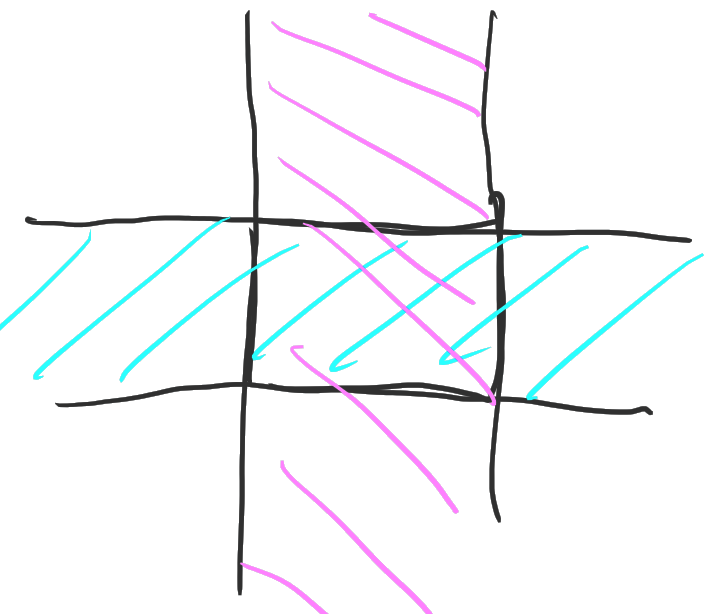
\includegraphics[width=0.25\textwidth]{tapes.png}
            \caption{Двумерные полоски.}
            \label{fig:tapes}
        \end{figure}

        Теперь посмотрим на промежутки:

        \begin{align*}
            I_1=\left[
            \begin{array}{ll}
                (a,\, b) \text{~--- открытое} \Rightarrow\in\FB(\R),\\
                \left[ a,\, b\right)=\bigcap\limits_{n=1}^{\infty} 
                \left(a-\dfrac{1}{n},\, b\right)\Rightarrow \in\FB(\R),\\ 
                \left( a,\, b\right]\text{~--- аналогично}\in\FB(\R),\\
                \left[a,\, b\right]\text{~--- дополнение к открытому}\Rightarrow\in\FB(\R).
            \end{array}
            \right .
        \end{align*}

        Аналогично множества $(I_1\times\R\times\ldots\times\R),\,
        (\R\times I_2\times\ldots\times \R),\,\ldots,\,
        (\R\times\R\times\ldots\times I_d)\in\FB(\R^d)$. А следовательно и их пересечение является
        борелевским множеством. 

        Итак, доказано, что $K_d\subset \FB(\R^d)\Rightarrow \sigma(K_d)\subset\FB(\R^d)$.

        Докажем теперь, что $\FB(\R^d)\subset \sigma(K_d)$. Так как 
        $\FB(\R^d)=\sigma(\tau)$ (см. определение), то достаточно доказать, что 
        $\tau\subset \sigma(K_d)$, в самом деле, если $\tau\subset \sigma(K_d)$, то 
        $\sigma(\tau)\subset \sigma(K_d)$ в силу минимальности $\sigma(\tau)$ по вложению.

        Пусть $U\in\tau$. Докажем, что $U\in\sigma(K_d)$.

        \begin{figure}[!ht]
            \centering
            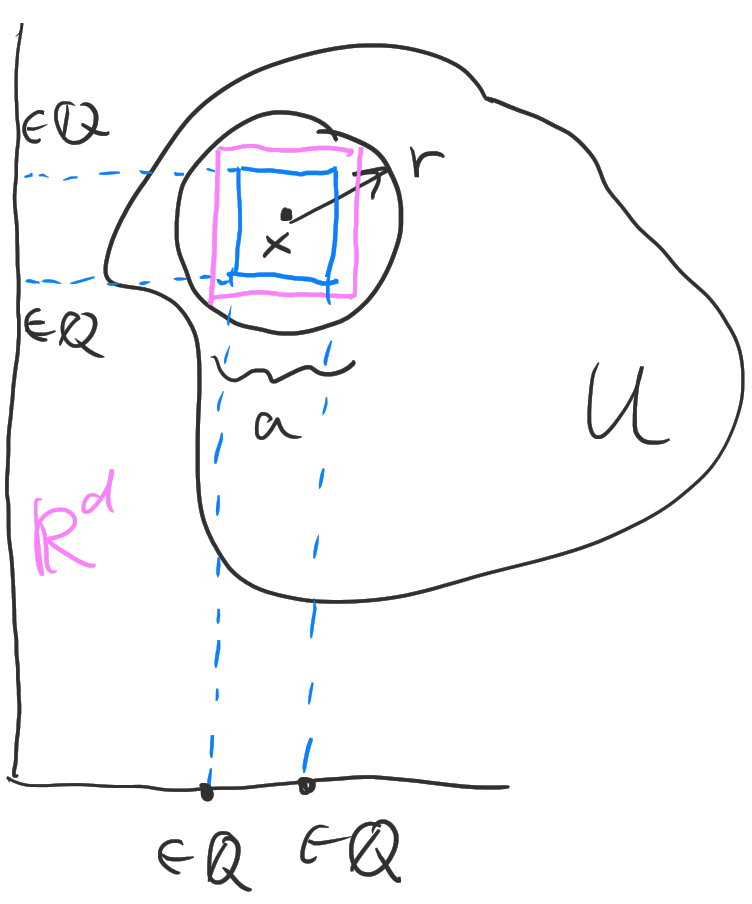
\includegraphics[width=0.6\textwidth]{upic.png}
            \caption{Множество $U$.}
            \label{fig:upic}
        \end{figure}

        $U$ открытое, поэтому $\forall x\in U\ \exists r>0:\ B_r(x)\subset U$, где $B_r(x)$~--- 
        $d$"=мерный шар радиуса $r$ с центром в точке $x$. Поймем какого размера должен быть 
        $d$"=мерный куб, чтобы его можно было вписать в данный шар. Должно выполнится следующее 
        неравенство: $\left(\dfrac{a}{2}\right)^2\cdot d\leqslant r^2$, где $a$~--- искомая сторона
        куба (неравенство следует из теоремы Пифагора: полудиагональ куба складывается из $d$ частей, 
        каждая длиной $\frac{a}{2}$). Откуда $a\leqslant \dfrac{2r}{\sqrt{d}}$. Таким образов любое 
        открытое множество можно представить в виде объединения таких кубиков (на рисунке \ref{fig:upic} это розовый квадрат),
        а кубики уже принадлежат семейству клеточных множеств.
        
        Но возникает проблема: такое объеденение кубиков может оказаться более чем счётным, поэтому сделаем финт ушами:
        сожмём кубик так, чтобы координаты его граней были рациональными (на рисунке это синий квадратик) и обзовем его $Q_x$.
        Множество таких кубов счётно, так как все такие кубы можно параметризовать точками $\Q^{2d}\Rightarrow$ данное семейство 
        счётно. 

        Тогда $\forall x\in U$ поставим в соответствие соответствующий куб $Q_x\subset B_r(x)\subset U$ и 
        $U=\bigcup\limits_{x\in U}\{x\}\subset \bigcup\limits_{x\in U}Q_x$~--- представимо в виде 
        не более чем счётного объединения, так как число кубов счётно и значит $U=\bigcup\limits_{x\in U}Q_x\in\sigma(K_d)$.

    \end{proof} 
\end{claim}

\subsection{Теорема Дынкина.}

\begin{definition}
    Семейство $\F\subset \CP(X)$ называется:
    \begin{enumerate}[label=\arabic*)]
        \item \mdef{$\pi$"=системой}, если $\forall A,\, B\in\F$ выполнено, что $A\cap B\in\F$;
        \item \mdef{$\lambda$"=системой}, если, во-первых, $\varnothing\in\F$, во-вторых,
        $\forall A\in\F$ выполнено, что $A^C\in\F$, а также для любых попарно непересекающихся 
        $D_1,\, \ldots,\, D_n,\,\ldots\in\F$ выполнено $\bigsqcup\limits_{k=1}^{\infty} D_k\in\F$.
    \end{enumerate}
\end{definition}

\begin{exercise}
    $\lambda$"=система в общем случае не всегда является $\pi$"=системой. Например, пусть 
    $X=\{1,\,2,\,3,\,4\}$ и 
    \[
        \F = \{\varnothing,\, X,\, \{1,\,2\},\, \{1,\,3\},\,\{1,\,4\},\,\{2,\,3\},\,\{2,\,4\},\,\{3,\,4\}\}.    
    \]
    Легко видеть, что это $\lambda$"=система, но не $\pi$"=система, так как $\F$ не замкнута относительно пересечения.
\end{exercise}

На прошлой лекции было доказано следующее утверждение (теперь в новой терминологии):
\begin{claim}
    $\F\subset\CP(X)$ является $\sigma$"=алгеброй тогда и только тогда, когда $\F$ 
    одновременно является $\pi$"=системой и $\lambda$"=системой.
\end{claim}

\begin{figure}[!ht]
    \centering
    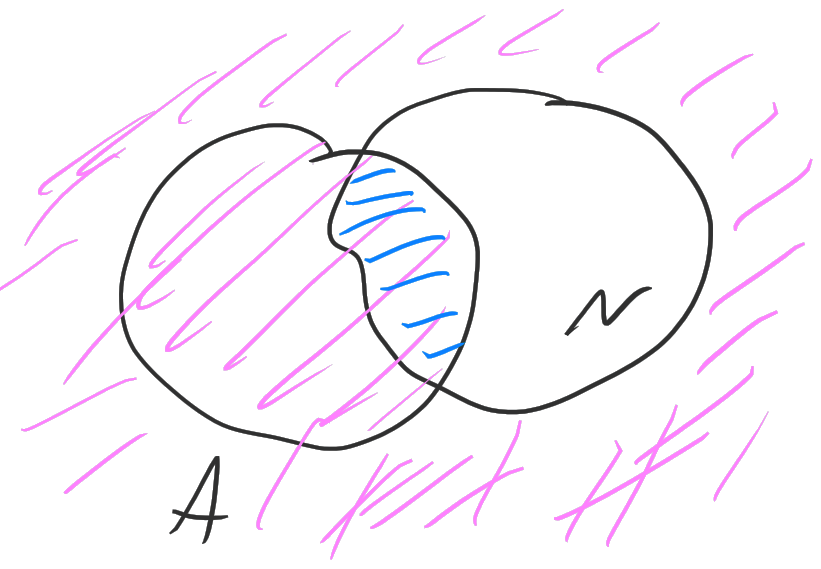
\includegraphics[width=0.5\textwidth]{sets.png}
    \caption{К теореме Дынкина (\ref{theorem:dynkin})}
    \label{fig:sets}
\end{figure}

\begin{theorem}[Дынкин]
    \label{theorem:dynkin}

    Пусть $\F\subset\CP(X)$~--- $\pi$"=система, $\CE\subset\CP(X)$~--- $\lambda$"=система и
    $\F\subset\CE$. Тогда $\sigma(\F)\subset\CE$ (равенство возможно).

    \begin{proof}
        Пусть $\CD\subset \CP(X)$~--- пересечение всех $\lambda$"=систем $\CG\subset\CP(X)$, 
        таких что $\F\subset\CG$. Докажем, что $\sigma(\F)\subset\CD$, для этого достаточно доказать, 
        что $\CD$ является $\sigma$"=алгеброй (снова в силу минимальности).

        Заметим, что $\CD$~--- $\lambda$"=система (доказывается так же как и факт о том, что пересечение сигма-алгебр является
        сигма-алгеброй). Тогда достаточно показать, что $\CD$~--- $\pi$"=система, то есть, что 
        $\forall M,\, N\in\CD$ выполняется, что $M\cap N\in\CD$.

        Введем обозначение: $\CH(M)=\{N\in\CD:\: M\cap N\in\CD\}$, где $M$~--- любой элемент $\CD$. То есть 
        условие о замкнутости по пересечению можно переформулировать так: $\forall M\in\CD$ выполнено $\CH(M)=\CD$.

        \begin{lemma}
            $\forall M\in\CD$ верно, что $\CH(M)$ является $\lambda$"=системой.

            \begin{proof}
                Во-первых, $\varnothing\in\CH(M)$, так как $\forall N\in\CD:\ \varnothing\cap N=\varnothing\in\CD$ по определению.

                Во-вторых, докажем, что $\CH(M)$ замкнуто относительно взятия дополнений. Пусть $A\in\CH(M)$. 
                Заметим, что
                \begin{equation}
                    \label{eq:lemmastate}
                    A\in\CH(M)\ \forall M\in\CD\Leftrightarrow\forall N\in\CD:\ A\cap N\in\CD.
                \end{equation}
                И в частности 
                \[
                    A^C\in\CH(M)\ \forall M\in\CD\Leftrightarrow\forall N\in\CD:\ A^C\cap N\in\CD.    
                \]
                Правое условие, в силу того, что $\CD$~--- $\lambda$"=система эквивалентно тому, что 
                $(A^C\cap N)^C\in\CD$ (из замкнутости по дополнению). Но $(A^C\cap N)^C=A\cup N^C=(A\cap N)\sqcup N^C\in\CD$ 
                (см. рис. \ref{fig:sets}). Итак, $A^C\in\CH(M)$.

                Докажем замкнутость относительно дизъюнктных объединений. Пусть 
                $A_1,\,\ldots,\,A_n,\,\ldots\in\CH(M)$ попарно не пересекаются. Тогда $\forall N\in\CD$:
                \[
                    \left(\bigsqcup_{n=1}^{\infty}A_n\right)\cap N=\bigsqcup_{n=1}^{\infty}\left(A_n\cap N\right)\in \CD,
                \]
                так как $A_n\cap N\in\CD$ (см. условие \eqref{eq:lemmastate}) и $\CD$~--- $\lambda$"=система.

            \end{proof}
        \end{lemma}

        Пусть $M\in\F\subset\CD$ (по построению). Зададимся вопросом: для каких $N\in\CD$ выполнено, что $M\cap N\in\CD$?
        Если $N\in\F$, то $M\cap N\in\F$, так как $\F$~--- $\pi$"=система. Поэтому $\forall N\in\F$
        выполнено $N\in\CH(M)$, то есть $\F\subset\CH(M)$, а значит $\CH(M)$~--- одна из $\lambda$"=систем, включающих в себя 
        $\F$, следовательно, в силу минимальности по вложению, $\CD\subset\CH(M)$ для $\forall M\in\F$, 
        то есть $\forall N\in\CD,\, \forall M\in\F$ выполнено $M\cap N\in\CD$. А значит $\forall N\in\CD$ выполнено $\F\subset\CH(N)$, и 
        снова в силу минимальности $\CD\subset \CH(N)$. Итак, $\forall N,\, M\in\CD$ выполнено $M\cap N\in\CD$.
        
    \end{proof}
\end{theorem}


\begin{task}{4}
	Рассмотрим функцию $\nu: \CP(\R) \rightarrow [0, +\infty]$ вида 
	$$
	\nu(A) = \#\{k \in \Z: [k, k+1)\cap A \neq \varnothing\},~ A \subset \R
	$$ 
где $\#B = n$ если множество $B$ состоит из $n \in \N_0$ элементов и $\#B = +\infty$ если множество $B$ бесконечно. Докажите, что $\nu$ является внешней мерой. Опишите все $\nu$-аддитивные множества.
\end{task}

\begin{solution}
	\begin{itemize}
		\item Докажем, что $\nu$ --- счетно-аддитивна:
		\begin{align*}
			\nu\left(\bigcup_{k=1}^{\infty} A_k\right) &= \#\left\{k \in \Z \mid 
			[k,k+1) \cap \bigcup_{k=1}^{\infty}A_k \neq \varnothing\right\} \leq \\ 
			&\leq \#\left\{\bigcup_{k=1}^{\infty}\left\{k\in \Z \mid 
			[k,k+1)\cap A_k \neq \varnothing \right\}\right\} = \sum_{k=1}^{\infty}\nu(A_k)
		\end{align*}
	
		\item 
		Докажем, что $\nu$-аддитивные множества это 
		$$
		A_\nu = \left\{\bigcup_{k=1}^{\infty}I_k\mid I_k \text{--- промежуток с целыми концами}\right\}
		$$
		Пусть $A \in A_\nu$, докажем, что 
		$$
		\nu(T) = \nu(T \cap A ) + \nu(T \cap A^c)
		$$
		\begin{equation}\label{task_4_f1}
		\nu(T\cap A) = \#\left\{k \in \Z \mid [k,k+1)\cap A\cap T \neq \varnothing \right\} = \#\left\{k \in \Z \mid ([k,k+1) \cap T)\cap A \right\}
		\end{equation}
		С другой стороны:
		\begin{equation}\label{task_4_f2}
		\nu(T\cap A^c) = \#\left\{k \in \Z \mid [k,k+1)\cap A^c\cap T \neq \varnothing \right\} = \#\left\{k \in \Z \mid ([k,k+1) \cap T)\cap A^c \right\}
		\end{equation}
		В силу того, $A$ и $A^c$ состоит из промежутков с целыми концами, то из \ref{task_4_f1}, \ref{task_4_f2}:
		$$
		\nu(T \cap A) + \nu(T \cap A^c) = \#\left\{k\in \Z \mid [k,k+1) \cap T \neq \varnothing \right\} = \nu(T)
		$$
		Пусть в $A_\nu$ есть множество $A$, точка границы замыкания которого --- не целая. 
		Тогда рассмотрим часть этого множества $A' \subset A$ без всех остальных укладывающихся в это множество
		единичных промежутков, $A' \in A_\nu$, так как $A_\nu$ --- сигма-алгебра. Не умаляя общности считаем, что 
		$$
		A' = [k,x), ~ x\notin \Z,~ x < k+1
		$$
		(случай отрезка рассматривается аналогично), тогда для $T = [k,k+1]$:
		$$
		1 = \nu(T) = \nu(T\cap A) + \nu(T \cap A^c) = 1 + 1 =2
		$$
		Таким образом $A_\nu$ действительно все $\nu$-аддитивные множества.
		\end{itemize}
	
	
\end{solution}


\newpage
\lecture{5}{Эргодичность и стационарность}
\begin{Def}
    Пусть процесс $\left\{ X(t), \ t \in T \right\}$ второго порядка, $[a,b]
    \subseteq T$; функция $g(t)$ непрерывна на этом отрезке; задано разбиение $a
    = t_0 < t_1 < \dots < t_{n-1} < t_n = b$, $\tau_i \in [t_{i-1}, t_i)$, а
    $\Delta = \dst \min_{i \in \{1, \dots, n\}}\left| t_i-t_{i-1} \right|$
    называется его мелкостью. Тогда если существует такая случайная величина
    $\eta$, что
    \begin{align*}
      & \sum_{i=1}^n g(\tau_i)(X(t_i)-X(t_{i-1})) \tosk{^{\Delta \to 0}_{n \to \infty}} \eta, \ \EE \eta^2 < \infty
    \end{align*}
    то эта величина называется \textbf{интегралом Римана-Стилтьеса в
      среднеквадратичном смысле от $g(t)$ по процессу $X(t)$ в пределах от $a$
      до $b$} (интегралом Римана-Стилтьеса в СК от $g(t)$ по $X(t)$ от $a$ до
    $b$) и записывается как
    \begin{align*}
      & \eta = \int_a^bg(t)dX(t)
    \end{align*}
\end{Def}
\begin{theorem}
    Критерий существования интеграла Римана-Cтилтьеса в среднеквадратичном
    смысле. (без доказательства)
    \\
    \begin{align*}
      & \exists \eta = \int_a^bg(t)dX(t) \Leftrightarrow \exists \int_a^b\int_a^b g(t)g(s)d^2K_x(t,s) = \lim_{^{\Delta t \to 0, n_t \to \infty}_{\Delta s \to 0, n_s \to \infty}} \sum_{i,j=0}^{n_t,n_s}g(\tau_i)g(\sigma_j)\left( K_X(t_{i+1},s_{j+1}) - \right. \\
      & \left. - K_X(t_{i},s_{j+1}) - K_X(t_{i+1},s_{j}) + K_X(t_{i},s_{j})\right) < \infty
    \end{align*}  
\end{theorem}
\begin{Note}
    ~
    \\
    Определение интеграла Римана-Стилтьеса в СК от $g$ по $X$ обобщается на
    несобственный случай следующим образом:
    \begin{align*}
      & \int_a^\infty g(t)dX(t) = \LIM{b \to \infty} \int_a^bg(t)dX(t)
    \end{align*}
    \begin{align*}
      & \int_{-\infty}^b g(t)dX(t) = \LIM{a \to -\infty} \int_a^bg(t)dX(t)
    \end{align*}
    \begin{align*}
      & \int_{-\infty}^\infty g(t)dX(t) = \LIM{^{a\to -\infty}_{b \to \infty}} \int_a^bg(t)dX(t)
    \end{align*}
\end{Note}
\begin{problem}
    ~
    \\
    Пусть $X'(t)$~--- СК-производная $X(t)$. Найти ее матожидание и
    корреляционную функцию.
\end{problem}
\begin{solution}
    ~
    \\
    Матожидание:
    \begin{align*}
      & \EE X'(t) = \EE \LIM{\varepsilon \to 0}\left( \frac{X(t+\varepsilon) - X(t)}{\varepsilon} \right) = \lim_{\varepsilon \to 0}\EE \left( \frac{X(t+\varepsilon) - X(t)}{\varepsilon} \right) = \frac{d}{dt}\EE X(t)
    \end{align*}
    Корреляционная функция:
    \begin{align*}
      & R_{X'}(t,s) = \EE \left( \left( X'(t) - \EE X'(t) \right)\left( X'(s) - \EE X'(s) \right) \right) = \EE \ \LIM{^{\varepsilon \to 0}_{\delta \to 0}}\left( \left( \frac{X(t+\varepsilon) - X(t)}{\varepsilon} - \right. \right. \\
      & \left. \left. - \frac{m_X(t+\varepsilon) - m_X(t)}{\varepsilon} \right)\left( \frac{X(s+\delta) - X(s)}{\delta} - \frac{m_X(s+\delta) - m_X(s)}{\delta} \right) \right) = \lim_{^{\varepsilon \to 0}_{\delta \to 0}} \frac{1}{\varepsilon \delta} \cdot \\
      & \cdot \left( R_X(t+\varepsilon, s+\delta) - R_X(t+\varepsilon, s) - R_X(t, s+\delta) + R_X(t, s)\right) = \frac{\partial^2 R_X}{\partial t \partial s}
    \end{align*}
\end{solution}
Аналогично можно вывести и формулы для интеграла.
\begin{Prop}
    ~
    \\
    Если $Y(t) = X'(t)$, то
    \begin{align*}
      & \EE Y(t) = \frac{d}{dt} \EE X(t), \ R_Y(t,s) = \frac{\partial^2 R_Y(t)}{\partial t \partial s}
    \end{align*}
    Если
    \begin{align*}
      & Y(t) = \int_a^t X(\tau) d\tau
    \end{align*}
    то
    \begin{align*}
      & \EE Y(t) = \int_a^t \EE X(\tau) d\tau, \ R_Y(t,s) = \int_a^s\int_a^t R_X(\tau, \sigma) d\tau d\sigma
    \end{align*}  
\end{Prop}
\section{Эргодические процессы}
\begin{Def}
    Пусть процесс $\left\{ X(t), \ t \geq 0 \right\}$ второго порядка имеет
    постоянное математическое ожидание $m$ и интегрируем в среднеквадратичном на
    любом отрезке $[0;T]$. Рассмотрим процесс
\begin{align*}
  & \left \langle X \right \rangle_T = \frac{1}{T} \int_0^T X(t) dt, \ T \geq 0
\end{align*}
Если $\left \langle  X \right \rangle_T \tosk{T \to \infty} m$, то процесс
$X(t)$ называется \textbf{эргодическим в среднеквадратичном смысле по
  математическому ожиданию} (эргодическим в СК по $\EE$).
\end{Def}
\begin{example}
    ~
    \\
    Процесс $\dst \frac{W(t)}{t}$ является эргодическим в СК по $\EE$.
\end{example}
\begin{Def}
    Процесс $\left\{ X(t), \ t \geq 0 \right\}$ называется \textbf{эргодическим в
      среднеквадратичном смысле по дисперсии} (эргодическим в СК по $D$), если
    процесс $Y(t) = \cent{X}^2(t) = \left( X(t) - \EE X(t) \right)^2$ эргодичен в
    СК по $\EE$.
\end{Def}
\begin{Note}
    \begin{align*}
      & \frac{1}{T} \int_0^T Y(t) dt \tosk{} \EE \cent{X}^2(t) = DX(t)
    \end{align*}
\end{Note}
\begin{Def}
    Процесс $\left\{ X(t), \ t \geq 0 \right\}$ называется \textbf{эргодическим в
      среднеквадратичном смысле по корреляционной функции} (эргодическим в СК по
    $R$), если $\forall \tau$ процесс $Z_\tau(t) = \cent{X}(t)\cent{X}(t+\tau)$
    эргодичен в СК по $\EE$.
\end{Def}
\begin{Note}
    \begin{align*}
      & \frac{1}{T} \int_0^T Z_\tau(t) dt \tosk{} \EE \left( \cent{X}(t)\cent{X}(t+\tau) \right) = R_X(t,\tau)
    \end{align*}
\end{Note}
\begin{theorem}
    Критерий эргодичности по математическому ожиданию.
    \\
    Процесс $\left\{ X(t), \ t \geq 0 \right\}$ второго порядка с постоянным
    математическим ожиданием $m$ и интегрируемый в СК на любом $[0;T]$ эргодичен
    в СК по $\EE$ тогда и только тогда, когда
    \begin{align*}
      & \lim_{T \to \infty} \frac{1}{T^2}\int_0^T \int_0^T R_x(t,s) dt ds = 0
    \end{align*}
\end{theorem}
\begin{proof}
    \begin{align*}
      & \EE \left( \frac{1}{T} \int_{0}^T X(t) dt - m\right)^2 = \EE \left( \frac{1}{T}\left( X(t)dt - \int_0^T m dt \right) \right)^2 = R_{\frac{1}{T}\int_0^T X(t) dt} (T,T) = \\
      & = \frac{1}{T^2}\int_0^T \int_0^T R_X(t,s) dt ds
    \end{align*}
    В силу равенства при эргодичности в СК по $\EE$ к нулю стремится первое, а
    значит, и последнее выражение; в случае стремления последнего выражения к
    нулю к нему стремится и первое, а значит, процесс эргодичен в СК по $\EE$.
\end{proof}
\begin{theorem}
    Достаточное условие эргодичности по математическому ожиданию.
    \\
    Процесс $\left\{ X(t), \ t \geq 0 \right\}$ второго порядка с постоянным
    математическим ожиданием $m$ и интегрируемый в СК на любом $[0;T]$ эргодичен
    в СК по $\EE$, если
    \begin{align*}
      & \lim_{\left| t - s \right| \to \infty} R_X(t,s) = 0
    \end{align*}
    \begin{align*}
      & \lim_{T \to \infty} \frac{1}{T} \max_{t \in [0;T]}R_X(t,t) = 0
    \end{align*}
\end{theorem}
\begin{proof}
    ~
    \\
    Выполнение данных условий влечет:
    \begin{align*}
      & \forall \varepsilon > 0 \ \exists T_0: \ \forall T = \left| t_2-t_1 \right|\geq T_0 \hookrightarrow \left| R_X(t_1,t_2) \right| < \varepsilon
    \end{align*}
    Положим
    \begin{align*}
      & G_1 = \left\{ (t_1,t_2) \in [0;T]^2: \ \left| t_2-t_1 \right| > T_0 \right\}
    \end{align*}
    \begin{align*}
      & G_2 = \left\{ (t_1,t_2) \in [0;T]^2: \ \left| t_2-t_1 \right| \leq T_0 \right\}
    \end{align*}
    и $S_1$, $S_2$ соответственно~--- их площади. Тогда
    \begin{align*}
      & \left| \frac{1}{T^2} \int_0^T\int_0^TR_X(t_1,t_2)dt_1dt_2 \right| = \frac{1}{T^2} \left( \us{G_1}{\int\int}R_X(t_1,t_2)dt_1dt_2 + \us{G_2}{\int\int}R_X(t_1,t_2)dt_1dt_2 \right) \leq \\
      & \leq \frac{1}{T^2} \left( \left| \us{G_1}{\int\int}R_X(t_1,t_2)dt_1dt_2 \right| + \left| \us{G_2}{\int\int}R_X(t_1,t_2)dt_1dt_2 \right| \right) \leq \frac{1}{T^2} \left( \us{G_1}{\int\int}\left| R_X(t_1,t_2) \right| dt_1dt_2 + \right. \\
      & \left. + \us{G_2}{\int\int}\left| R_X(t_1,t_2) \right| dt_1dt_2 \right) \leq \frac{1}{T^2} \left( \varepsilon S_1 + \max_{G_2}\left| R_X(t_1,t_2) \right| S_2 \right) \leq \varepsilon + \frac{\dst \max_{G_2}\left| R_X(t_1,t_2) \right| S_2}{T^2} \leq \\
      & \leq \varepsilon + \frac{2T_0 \dst \max_{G_2}\left| R_X(t_1,t_2) \right|}{T} \leq \varepsilon + \frac{2T_0 \sqrt{\dst \max_{G_2} R_X(t_1,t_1)R_X(t_2,t_2)}}{T} \leq \varepsilon + \frac{2T_0 \dst \max_{t \in [0;T]} R_X(t,t)}{T} \To{T \to \infty} 0
    \end{align*}
    А такой предел указан в критерии эргодичности в СК по $\EE$.
\end{proof}
\begin{Note}
    ~
    \\
    Если у процесса дисперсия растет медленнее, чем линейно, то для эргодичности
    достаточно проверить только первое условие из достаточного.
    \\
    То же верно, если
    \begin{align*}
      & \exists c: \ \forall t \ \EE X^2(t) < c
    \end{align*}
\end{Note}
\section{Стационарные процессы.}
Стационарные процессы имеют не зависящие от времени распределения сечений,
многомерные распределения, зависящие лишь от разности моментов времени, и
описывают установившиеся во времени явления.
\begin{Def}
    Процесс $\left\{ X(t), \ t \in T \right\}$ называется \textbf{стационарным в
      узком смысле}, если все его конечномерные распределения не зависят от сдвига
    по времени на одну и ту же величину, т.~е.
    \begin{align*}
      & \forall t_1, \dots, t_n \in T, \ \forall \tau: \ t_1+\tau, \dots, t_n + \tau \in T \hookrightarrow \\
      & F_X(x_1, \dots, x_n; t_1, \dots, t_n) = F_X(x_1, \dots, x_n; t_1 + \tau, \dots, t_n+\tau)
    \end{align*}
    или, что то же самое, векторы
    \begin{align*}
      & \left[ \begin{matrix}
              X(t_1) \\
              X(t_2) \\
              \dots \\
              X(t_n)
          \end{matrix} \right], \  \left[ \begin{matrix}
              X(t_1+\tau) \\
              X(t_2+\tau) \\
              \dots \\
              X(t_n+\tau)
          \end{matrix} \right]
    \end{align*}
    одинаково распределены.
\end{Def}
\begin{example}
    ~
    \\
    Одномерное распределение:
    \begin{align*}
      F_X(x,t) = F_X(x, t + \tau) \Rightarrow \EE X(t) = m_X = const , \ D X(t) = \sigma^2 = const, \ \dots
    \end{align*}
    Все моменты постоянны во времени.
    Двумерное распределение:
    \begin{align*}
      F(x_1,x_2; t_1, t_2) = F_X(x_1, x_2; t_1 + \tau, t_2 + \tau) \Rightarrow R_X(t_1,t_2) = R_X(t_1+\tau, t_2+\tau) = R_X(0, t_2-t_1)
    \end{align*}
    Корреляционная функция зависит только от разности моментов времени.
\end{example}
\begin{Def}
    Процесс $\left\{ X(t), \ t \in T \right\}$ называется \textbf{стационарным в
      широком смысле}, если его математическое ожидание постоянно во времени, а
    корреляционная функция зависит от своих аргументов только через их разность, т.~е.
    \begin{align*}
      & \EE X(t) = m = const, \ R_X(t,s) = R(t-s)
    \end{align*}
\end{Def}
\begin{Prop}
    ~
    \\
    Если процесс второго порядка стационарен в узком смысле, то он стационарен и
    в широком смысле, но не наоборот.
\end{Prop}
\begin{Proof}
    ~
    \\
    Как было показано в примере выше, условия определения широкого смысла выполняются.
\end{Proof}
\begin{example}
    ~
    \\
    Контрпример к обратному утверждению: процесс
    \begin{align*}
      & Z(t) = X\cos t + Y \sin t, t \geq 0, \ X,Y \ \IID, \ \PP\{X = 1\} = \PP\{X = -1\} = \frac{1}{2}
    \end{align*}
    стационарен в широком, но не узком смысле.
\end{example}
\begin{theorem}
    ~
    \\
    Нормальный процесс стационарен в широком смысле тогда и только тогда, когда
    он стационарен в узком смысле.
\end{theorem}
\begin{Proof}
    ~
    \\
    Нормальный процесс является процессом второго порядка, а значит,
    необходимость очевидна.
    \\
    Пусть теперь $X(t)$ стационарен в широком смысле. Возьмем произвольное
    сечение (нормальный случайный вектор)
    \begin{align*}
      & X = \left[ \begin{matrix}
              X(t_1) \\
              \dots \\
              X(t_n)
          \end{matrix} \right] \Rightarrow \varphi_X(s) = \exp \left( is^tm - \frac{1}{2}s^TRs \right), \ s = \left( s_1, \dots, s_n \right)
    \end{align*}
    При сдвиге всех $t_i$ на одну и ту же величину $\tau$ ни $m$, ни $R$ не
    изменились, тогда и $\varphi_X(s)$ не изменится, а она задает многомерные
    распределения. Они не меняются, значит, стационарность в узком смысле
    выполняется.
\end{Proof}
\begin{Note}
    ~
    \\
    Для стационарного процесса достаточно лишь первого из условий эргодичности.
    Второе выполняется автоматически.
\end{Note}
\begin{task}{9}
	Доказать, что всякое измеримое по Лебегу множество, мера которого строго положительна, содержит неизмеримое множество.
\end{task}


\begin{solution}
Вот тут была написана хуйня, я запилю норм решение
\end{solution}


\begin{linkthm}{https://youtu.be/MXQbqUweyEw?t=4}[Минимальное свойство сумм Фурье]\ \\
	Если $\{e_k\}$ --- ортогональная система ненулевых эдементов евклидова пространства $E$, то $(\forall f\in E)(\forall c_1,\ldots, c_N \in \R)\|f-\sum\limits_{k=1}^N c_k e_k\|\geqslant \|f-\sum\limits_{k=1}^N f_ke_k\|$, где $\{f_k\}$ --- коэффициенты Фурье для $f$, причем равенство равносильно $c_k=f_k, k=1,\ldots, N$.
\end{linkthm}
\begin{proof} Рассмотрим квадрат нормы
\begin{multline*}
\|f-\sum\limits_{k=1}^N c_ke_k\|^2=<f-\sum\limits_{k=1}^Nc_ke_k, f-\sum\limits_{k=1}^Nc_ke_k>=\\=<f,f>-2\sum\limits_{k=1}^Nc_k<f,e_k>+\sum\limits_{k=1}^N\sum\limits_{l=1}^N c_kc_l<e_k,e_l>=\\=\left[f_k=\frac{<f,e_k>}{\|e_k\|^2}; <e_k,e_l>=0, k\ne l\right]=\\=<f,f>-2\sum\limits_{k=1}^Nf_kc_k\|e_k\|^2+\sum\limits_{k=1}^Nc_k^2\|e_k\|^2=\\=\left[\text{прибавим и вычтим } \sum\limits_{k=1}^Nf_k^2\|e_k\|^2\right]=\\=\|f\|^2-\sum\limits_{k=1}^Nf_k^2\|e_k\|^2+\sum\limits_{k=1}^N(f_k^2-2f_kc_k+c_k^2)\|e_k\|^2\geqslant \\ \geqslant \|f\|^2-\sum\limits_{k=1}^Nf_k^2\|e_k\|^2=\|f-\sum\limits_{k=1}^Nf_ke_k\|^2.
\end{multline*}
\end{proof}

\begin{corollary}[Тождество Бесселя]
	Если $\{e_k\}$ --- ортогональная система ненулевых элементов евклидова  пространства $E$, то $(\forall f\in E) \|f-\sum\limits_{k=1}^N f_ke_k\|^2=\|f\|^2-\sum\limits_{k=1}^N f_k^2\|e_k\|^2$, где $f_k$ --- коэффициенты Фурье $f$.
\end{corollary}

\begin{corollary}[Неравенство Бесселя]
	Если $\{e_k\}_{k=1}^\infty$ --- ортогональная система ненулевых элементов евклидова  пространства $E$, то $(\forall f\in E) \sum\limits_{k=1}^N f_k^2\|e_k\|^2\leqslant \|f\|^2$, где $f_k$ --- коэффициенты Фурье $f$.
\end{corollary}

\begin{linkthm}{https://youtu.be/MXQbqUweyEw?t=845}[О полноте ортогональной системы функций]\ \\
	Если $\{e_k\}_{k=1}^\infty$ --- ортогональная система ненулевых элементов евклидова пространства $E$, то $(\forall f\in E)$ следующие утверждения эквивалентны:
	\begin{enumerate}
		\item $(\forall\varepsilon>0)(\exists T=\sum\limits_{k=1}^Nc_ke_k) \|f-T\|<\varepsilon$.
		\item $f=\sum\limits_{k=1}^\infty f_ke_k$.
		\item $\|f\|^2=\sum\limits_{k=1}^\infty f_k^2\|e_k\|^2$ (равенство Парсеваля).
	\end{enumerate}
\end{linkthm}
\begin{proof}
	TODO%$\emph{1)}\Leftrightarrow\emph{2)}$
\end{proof}

\begin{corollary}
	Если $\{e_k\}_{k=1}^\infty$ --- ортогональная система ненулевых элементов евклидова пространства $E$, то следующие утверждения эквивалентны:
	\begin{enumerate}
		\item $\{e_k\}_{k=1}^\infty$ --- полная система в $E$.
		\item $(\forall f\in E) f=\sum\limits_{k=1}^\infty f_ke_k$.
		\item $(\forall f\in E) \|f\|^2=\sum\limits_{k=1}^\infty f_k^2\|e_k\|^2$.
	\end{enumerate}
\end{corollary}

\begin{linkthm}{https://youtu.be/MXQbqUweyEw?t=1454}[Рисса-Фишера]\ \\
	Если $\{e_k\}_{k=1}^\infty$ --- ортогональная система ненулевых элементов гильбертова пространства $H$ и $\{\alpha_k\}_{k=1}^\infty$ --- последовательность действительных чисел такая, что $\sum\limits_{k=1}^\infty \alpha_k^2\|e_k\|^2$ сходится, то ряд $\sum\limits_{k=1}^\infty \alpha_ke_k$ сходится к некоторому $f\in H$.
\end{linkthm}
\begin{proof}
	TODO
\end{proof}

\begin{corollary}
	Если $\{e_k\}_{k=1}^\infty$ --- ортогональная система ненулевых элементов гильбертова пространства $H$, то $(\forall f\in H)$ ряд Фурье сходится к $f_0\in H: \sum\limits_{k=1}^\infty f_ke_k=f_0$ и $<f-f_0,e_j>=0 (\forall j\in \N)$.
\end{corollary}
\begin{proof}
TODO
\end{proof}

\begin{Def}
	Система $\{e_k\}_{k=1}^\infty$ называется замкнутой в евклидовом пространстве $E$ (по Банаху, в банаховом пространстве тотальной, в $C$ и $L_p$ --- полной), если из ${<f,e_k>=0}\\{(\forall k\in \N)}\Rightarrow f=0$.
\end{Def}

\begin{linkthm}{https://youtu.be/MXQbqUweyEw?t=2358}[Полнота и замкнутость ортогональной системы, их связь]\ \\
	$\{e_k\}_{k=1}^\infty$ --- замкнутая система в гильбертовом пространстве $\Leftrightarrow$ она полная.
\end{linkthm}
\begin{proof}
	TODO
\end{proof}

Рассмотрим пространство $L_{2\pi}^2$, которое состоит из $2\pi$-периодических функций, принадлежащих $L^2[-\pi,\pi]$. Оно гильбертово. Рассмотрим ортогональную систему $\{e_k\}_{k=1}^\infty=\{\frac{1}{2},\cos x,\sin x,\cos2x, \sin 2x,\ldots\}$.
TODO

\begin{linkthm}{https://youtu.be/MXQbqUweyEw?t=3890}[Хаусдорфа-Юнга]\ \\
	Пусть $1<p\leqslant 2$.
	\begin{enumerate}
		\item Если последовательность $a_0, \{a_n,b_n\}_{n=1}^\infty\in l_p$(определение $l_p$ смотри выше), то она является последовательностью коэффициентов тригонометрического ряда Фурье функции $f\in L_q^{2\pi}$, где $\frac{1}{p}+\frac{1}{q}=1$.
		\item Если $f\in L_p^{2\pi}$, то последовательность коэффициентов ее тригонометрического ряда Фурье принадлежит $l_q$, где $\frac{1}{p}+\frac{1}{q}=1$.
	\end{enumerate}
\end{linkthm}
\begin{note}
	Результаты этого параграфа справедливы и в унитарных пространствах.
\end{note}









\newpage
\section{Глава 12. Интегралы, зависящие от параметра.}
\subsection{Собственные интегралы, зависящие от параметра.}
\begin{linkthm}{https://youtu.be/tCE6Kl7Sy2s?t=96}
	Пусть $\forall \alpha\in A\subset \R^n$ функция $f_{1,\alpha}(x)=f(x,\alpha)$ суммируема на $E\subset\R^m$, функция $f_{2,x}(\alpha)=f(x,\alpha)$ при почти всех $x\in E$ непрерывна в $\alpha_0\in E$, и при почти всех $x\in E, \forall\alpha\in A\  |f(x,\alpha)|\leqslant\varphi(x)$, где $\varphi(x)$ суммируемая на $E$. Тогда $F(\alpha)=\int\limits_{E}f(x,\alpha)d\mu(x)$ непрерывна в $\alpha_0$.
\end{linkthm}
\begin{proof}
	Рассмотрим произвольную последовательность Гейне $\forall\{\alpha_n\}_{n=1}^\infty\subset A,\\ \lim\limits_{n\to\infty}\alpha_n=\alpha_0$. Тогда по условию $\lim\limits_{n\to\infty}f(x,\alpha_n)=f(x,\alpha_0)$ при почти всех $x\in E$. Также $|f(x,\alpha_n)|\leqslant \varphi(x) (\forall n\in\N)$ для почти всех $x\in E$. Тогда $\int\limits_E f_{1,\alpha_n}(x)d\mu(x)\underset{n\to\infty}{\overset{\text{по т. Лебега}}{\longrightarrow}}\int\limits_{E}f(x,\alpha_0)d\mu(x)$. Но это и означает, что $F(\alpha_n)=\int\limits_{E}f(x,\alpha_n)d\mu(x)=\int\limits_E f_{1,\alpha_n}(x)d\mu(x)\underset{n\to\infty}{\longrightarrow} F(\alpha_0)$ и ввиду произвольного выбора последовательности Гейне получаем непрерывность.
\end{proof}

\begin{corollary}
	Если $f$ непрерывна на $[a,b]\times [c,d]$, то $\int\limits_a^bf(x,y)dx=F(y)$ непрерывна на $[c,d]$.
\end{corollary}

\begin{linkthm}{https://youtu.be/tCE6Kl7Sy2s?t=686}
	Пусть $f_{1,\alpha}(x)=f(x,\alpha)$ при всех $\alpha\in U(\alpha_0)\subset\R$ суммируема на $E\subset \R^m$ вместе с $\frac{\partial f(x,\alpha)}{\partial \alpha}$, и при почти всех $x\in E, \forall\alpha\in U(\alpha_0): \left|\frac{\partial f(x,\alpha_0)}{\partial\alpha}\right|\leqslant\varphi(x)$, где $\varphi(x)$ суммируема на $E$. Тогда $F'(\alpha_0)=\int\limits_E\frac{\partial f(x,\alpha_0)}{\partial\alpha}d\mu(x)$, где $F(\alpha)=\int\limits_E f(x,\alpha)d\mu(x)$.
\end{linkthm}

\begin{proof}
	Возьмем произвольную последовательность $\forall\{\alpha_n\}_{n=1}^\infty\subset\overset{\circ}{U}(\alpha_0),\\ \lim\limits_{n\to\infty}\alpha_n=\alpha_0$. Тогда частная производная $\left|\frac{f(x,\alpha_n)-f(x,\alpha_0)}{\alpha_n-\alpha_0}\right|\overset{\text{т. Лагранжа о сред.}}{=}\left|\frac{\partial f(x,\xi_n(x))}{\partial\alpha}\right|\leqslant\varphi(x)$. По теореме Лебега $\lim\limits_{n\to\infty}\int\limits_E\frac{f(x,\alpha_n)-f(x,\alpha_0)}{\alpha_n-\alpha_0}d\mu(x)=\int\limits_E\frac{\partial f(x,\alpha_0)}{\partial\alpha}d\mu(x)$. Пользуемся линейностью интеграла Лебега и замечаем, что $\frac{F(\alpha_n)-F(\alpha_0)}{\alpha_n-\alpha_0}=\int\limits_E\frac{f(x,\alpha_n)-f(x,\alpha_0)}{\alpha_n-\alpha_0}d\mu(x)$. То есть мы установили что существует предел $\lim\limits_{n\to\infty}\frac{F(\alpha_n)-F(\alpha_0)}{\alpha_n-\alpha_0}=\int\limits_E\frac{\partial f(x,\alpha_0)}{\partial\alpha}d\mu(x)$. Это в точности и означает, что существует $F'(\alpha_0)=\int\limits_E\frac{\partial f(x,\alpha_0)}{\partial\alpha}d\mu(x)$.
\end{proof}
\begin{corollary}
Если $f(x,y)$ и $\frac{\partial f}{\partial y}$ непрерывны на $[a,b]\times[c,d]$, то справедливо правило Лейбница  $\forall y\in [c,d]:\frac{d}{dy}\left(\int\limits_a^bf(x,y)dx\right)=\int\limits_a^b\frac{\partial f(x,y)}{\partial y}dx$.
\begin{proof}
Из того что $\frac{\partial f}{\partial y}$ непрерывна на компакте $\Rightarrow \left|\frac{\partial f}{\partial y }(x,y)\right|\leqslant C$, значит в качестве функции $\varphi(x):=C$, и все условия теоремы 12.1.2 выполены и мы можем дифференцировать.
\end{proof}
\begin{corollary}[из следствия]
Если $f$ и $\frac{\partial f}{\partial y}$ непрерывны на $[a,b]\times[c,d]$, и $a\leqslant \varphi(y)\leqslant\psi(y)\leqslant b\  \forall y\in [c,d]$, где $\varphi, \psi$ дифференцируемы на $[c,d]$, то $$\frac{d}{dy}\left(\int\limits_{\varphi(y)}^{\psi(y)}f(x,y)dx\right)=\int\limits_{\varphi(y)}^{\psi(y)}\frac{df}{dy}(x,y)dx+f(\psi(y),y)\cdot\psi'(y)-f(\varphi(y),y)\cdot\varphi'(y).$$
\end{corollary}
\begin{proof}
Рассмотрим функцию $F(x,y,u,v)=\int\limits_u^v f(x,y)dx$: она  непрерывна, как функция параметра $y\ \forall u,v$; дифференцируема по $y$, кроме того она дифференцируема по $u$ и по $v$ как следствие интеграла с переменным верхним пределом, подставляем вместо $u,v$ дифференцируемые функции $\varphi, \psi$ и применяем правило дифференцирования сложной функции многих переменных.
\end{proof}
\end{corollary}

\subsection{Несобственные интегралы Римана, зависящие от параметра.}

Пусть $f(x,y)\in \mathcal{R}[a,\widetilde{b}]\ \forall\widetilde{b}<b\ \forall y\in A\subset \R$. Тогда несобственным интегралом Римана называется
\begin{equation}
	\int\limits_a^b f(x,y)dx=\lim\limits_{\widetilde{b}\to b(-0)}\int\limits_a^{\widetilde{b}} f(x,y)dx.
\end{equation}
\begin{Def}
	Несобственный интеграл $(1)$ сходится равномерно на $A$, если $(\forall\varepsilon>0)(\exists B\in(a,b))(\forall B'\in(B,b))(\forall y\in A)\left|\int\limits_{B'}^b f(x,y)dx\right|<\varepsilon$.
\end{Def}

\begin{linkthm}{https://youtu.be/tCE6Kl7Sy2s?t=2769}[Критерий Коши равномерной сходимости несобственных интегралов, зависящих от параметра]\ \\
	Несобственный интеграл $(1)$ сходится равномерно на $A\Leftrightarrow \left(\forall\varepsilon>0\right)(\exists B\in(a,b))(\forall B', B'':\\ B<B'<B''<b)(\forall y\in A)\left|\int\limits_{B'}^{B''}f(x,y)dx\right|<\varepsilon$.
\end{linkthm} 
\begin{proof}
	Пусть интеграл $\int\limits_a^bf(x,y)dx$ равномерно сходится по параметру $y\in A$. По определению $(\forall\varepsilon>0)(\exists B\in(a,b))(\forall B'\in(B,b))(\forall y\in A)\left|\int\limits_{B'}^b f(x,y)dx\right|<\frac{\varepsilon}{2}$. При произвольных $B', B'':B<B'<B''<b$ получим неравенство $\left|\int\limits_{B'}^{B''}f(x,y)dx\right|=\left|\int\limits_{B'}^bf(x,y)dx-\int\limits_{B''}^bf(x,y)dx\right|\leqslant \left|\int\limits_{B'}^bf(x,y)dx\right|+\left|\int\limits_{B''}^bf(x,y)dx\right|<\frac{\varepsilon}{2}+\frac{\varepsilon}{2}=\varepsilon$.
	
	Пусть $\left(\forall\varepsilon>0\right)(\exists B\in(a,b))(\forall B', B'': B<B'<B''<b)(\forall y\in A)\left|\int\limits_{B'}^{B''}f(x,y)dx\right|<\varepsilon$. Зафиксируем $y\in A$, тогда по критерию Коши сходимости несобственных интегралов получаем, что $\int\limits_a^bf(x,y)dx$ сходится. В неравенстве $\left|\int\limits_{B'}^{B''}f(x,y)dx\right|<\varepsilon$ устремим $B''$ к $b$, получим, что $(\forall B'\in(B,b))(\forall y\in A)\left|\int\limits_{B'}^{b}f(x,y)dx\right|\leqslant\varepsilon$ это и означает равномерную сходимость интеграла.
\end{proof}

\begin{corollary}[Признак сравнения]
	Если $|f(x,y)|\leqslant g(x,y), f, g$ удовлетворяют условиям определения несобственного интеграла Римана и $\int
	\limits_a^b g(x,y)dx$ равномерно сходится на $A$, то $\int\limits_a^b f(x,y)dx$ равномерно сходится на $A$.
\end{corollary}
\begin{corollary}[Признак Вейершрасса]
	Если $|f(x,y)|\leqslant g(x), f, g$ удовлетворяют условиям определения несобственного интеграла Римана и $\int
	\limits_a^b g(x)dx$ сходится на $A$, то $\int\limits_a^b f(x,y)dx$ равномерно сходится на $A$.
\end{corollary}

\begin{linkthm}{https://youtu.be/tCE6Kl7Sy2s?t=3664}[Признак Дирихле равномерной сходимости несобственных интегралов Римана, зависящих от параметра]\ \\
	Пусть
	\begin{enumerate}
		\item $f\in\mathcal{R}[a, \widetilde{b}](\forall\widetilde{b}\in(a,b))(\forall y\in A)$ и $(\forall y\in A)\left|\int\limits_a^x f(t,y)dt\right|\leqslant C$ (равномерная ограниченность первообразной),
		\item $g(x,y)$ монотонно сходится к 0 при $x\to b(-0)$ равномерно по $y\in A$.
	\end{enumerate}
Тогда $\int\limits_a^b f(x,y)\cdot g(x,y)dx$ равномерно сходится на $A$.
\end{linkthm}

\begin{proof}
	Рассмотрим интеграл и воспользуемся формулой Бонне: $$\int\limits_{B'}^{B''}f(x,y)\cdot g(x,y)dx = g(B',y)\int\limits_{B'}^{\xi(y)}f(x,y)dx+g(B'',y)\int\limits_{\xi(y)}^{B''}f(x,y)dx.$$
	Так как $g(x,y)\underset{x\to b(-0)}{\rightrightarrows} 0$, то есть $(\forall\varepsilon>0)(\exists B\in(a,b))(\forall x\in (B,b))(\forall y\in A)\ |g(x,y)|<\frac{\varepsilon}{4C}$. Оценим $\left|\int\limits_{B'}^{\xi(y)}f(x,y)dx\right|=\left|\int\limits_{a}^{\xi(y)}f(x,y)dx-\int\limits_{a}^{B'}f(x,y)dx\right|\leqslant 2C\Rightarrow \int\limits_{B'}^{B''}f(x,y)\cdot g(x,y)dx\leqslant \varepsilon$.
\end{proof}

\begin{linkthm}{https://youtu.be/tCE6Kl7Sy2s?t=4226}[Признак Абеля равномерной сходимости несобственных интегралов Римана, зависящих от параметра]\ \\
Пусть
\begin{enumerate}
	\item $f\in\mathcal{R}[a, \widetilde{b}](\forall\widetilde{b}\in(a,b))(\forall y\in A)$ и $\int\limits_a^b f(x,y)dx$ равномерно сходится на $A$,
	\item $g(x,y)$ монотонна по $x\ \forall y\in A$ и $(\forall x\in (a,b))(\forall y\in A)|g(x,y)|\leqslant C$.
\end{enumerate}
Тогда $\int\limits_a^b f(x,y)\cdot g(x,y)dx$ равномерно сходится на $A$.
\end{linkthm}

\begin{proof}
	Рассмотрим интеграл и воспользуемся формулой Бонне:
	\begin{multline*}
		\left|\int\limits_{B'}^{B''}f(x,y)\cdot g(x,y)dx\right| \leqslant\left|g(B',y)\right|\cdot\left|\int\limits_{B'}^{\xi(y)}f(x,y)dx\right|+\left|g(B'',y)\right|\cdot\left|\int\limits_{\xi(y)}^{B''}f(x,y)dx\right|<\\<C\cdot\frac{\varepsilon}{2C}+C\cdot\frac{\varepsilon}{2C}=\varepsilon.
	\end{multline*} 
\end{proof}


















\begin{task}{9}
	Является ли семейство 
	$$
	\F = \{A \times \R : A \subset \R\} \cup \{\R \times B : B \subset \R \}
	$$
	
	\begin{itemize}
		\item[a)] $\pi$-системой;
		\item[б)] $\lambda$-системой подмножеств множества $X = \R^2$
	\end{itemize}
\end{task}

\begin{solution}
	\begin{enumerate}
		\item[a)] Докажем, что $\F$ --- не $\pi$-система, действительно:
		$$
		\{\R\times A\} \in \F, \{A \times \R\} \in \F
		$$
		но, так как $A \subsetneq \R$
		$$
		\{\R \times A\} \cap \{A \times R\} = \{A \times A\} \notin \F 
		$$
		Таким образом $\F$ --- не $\pi$-система
		\item[б)] Докажем, что $\F$ --- $\lambda$ -система:
		\begin{itemize}
			\item $\varnothing \in \F$
			\item $\forall A \in \F$ если $A = \{B \times \R \}$, где $B \subset \R$ имеем: 
			$$
			A^c = \{B^c \times \R \} \in \F
			$$ 
			Аналогично для $A = \{\R \times B\}$
			\item Пусть $\left\{ D_k \right\}_{k=1}^{\infty} \subset \F$ --- дизъюнктное семейство, тогда есть два случая: 
			$$
			D_i = \{A_i \times \R \}; ~ D_i = \{\R \times A_i\}
			$$
			В каждом случае $\left\{A_i\right\}_{i=1}^{\infty}$ --- дизъюнктные семейства.
			Тогда 
			$$
			\bigcup_{k=1}^{\infty} D_k = 
			\left[ 
			\begin{gathered} 
				\vspace{3px}
				\bigcup_{n=1}^{\infty} \{A_n \times \R\} = \{A_N \times \R \} \in \F
				\\ 
				\bigcup_{m=1}^{\infty} \{\R \times A_m\} = \{\R \times A_M\} \in \F
				\vspace{3px}
				\\ 
			\end{gathered} 
			\right.
			$$
		\end{itemize}
	Таким образом $\F$ --- $\lambda$-система.
	\end{enumerate}
	
\end{solution}
\begin{linkthm}{https://youtu.be/U6GjvhvickE?t=397}[Формула Гаусса-Эйлера]\ \\
	Для любых $\alpha >0:\ \Gamma(\alpha)=\lim\limits_{n\to\infty}n^\alpha\frac{(n-1)!}{\alpha(\alpha+1)\cdot\ldots\cdot(a+n-1)}$.
\end{linkthm}
\begin{proof}
	TODO
\end{proof}


\begin{linkthm}{https://youtu.be/U6GjvhvickE?t=1408}[Формула Валлиса]\ \\
	Для любых $\alpha \in\R, |\alpha|<1: \frac{\sin\alpha\pi}{\alpha\pi}=\prod\limits_{n=1}^\infty (1-\frac{\alpha^2}{n^2})$.
\end{linkthm}
\begin{proof}
	TODO
\end{proof}

\begin{linkthm}{https://youtu.be/U6GjvhvickE?t=2680}[Формула дополнения]\ \\
	Для любых $\alpha , 0<\alpha<1: \Gamma(\alpha)\Gamma(1-\alpha)=\frac{\pi}{\sin\alpha\pi}$.
\end{linkthm}
\begin{proof}
	TODO
\end{proof}
\newpage
\lecture{11}{Непрерывные цепи Маркова}
\section{Непрерывные цепи Маркова}
\subsection{Непрерывные цепи Маркова}
\begin{Def}
    Случайная функция
    \begin{align*}
      & X(t), \ t \geq 0, \ S \subseteq \ZZ, \ \left| S \right| \leq \infty
    \end{align*}
    со свойством
    \begin{align*}
      & \forall n \geq 1, \ \forall m_0 < m_1 < \dots < m_n \ \PP\left( X(t_n) = x_n \mid X(t_{n-1}) = x_{n-1}, \dots, X(t_0) = x_0 \right) = \\
      & = \PP\left( X(t_{n}) = x_n \mid X(t_{n-1}) = x_{n-1}\right)
    \end{align*}
    где эти вероятности определены, называется \textbf{непрерывной марковской
      цепью (НМЦ)}.
\end{Def}
\begin{Def}
    Если состояний конечное число, то НМЦ называется \textbf{конечной}, иначе \textbf{счетной}.
\end{Def}
\begin{Def}
    Вероятность
    \begin{align*}
      & p_{ij}(t_1,t_2) = \PP \left( X(t_1)=j \mid X(t_2) = i\right)
    \end{align*}
    назовем \textbf{вероятностью перехода из из состояния $i$ в момент $t_1$ в
      состояние $j$ в момент $t_2$} ($t_1 \leq t_2$).
\end{Def}
\begin{Def}
    Матрица
    \begin{align*}
      & P(t_1,t_2) = \left| \left| \begin{matrix} p_{ij}(t_1,t_2) \end{matrix} \right| \right|
    \end{align*}
    называется \textbf{матрицей перехода цепи от момента $t_1$ к моменту $t_2$}
    ($t_1 \leq t_2$).
\end{Def}
\textbf{Свойства}
\begin{enumerate}
    \item $\forall i \in S, \ 0 \leq s \leq t \ \dst \sum_{j \in S} p_{ij}(s,t) = 1$
    \item $\forall i \in S, \ 0 \leq t \ p_{ii}(t,t) = 1$
    \item $\forall i \neq j \in S, \ 0 \leq t \ p_{ij}(t,t) = 0$
\end{enumerate}
\begin{theorem} Уравнение Колмогорова-Чепмена
    \\
    Пусть $t_1 < t < t_2$. Тогда выполняется
    \begin{align*}
      & P(t_1,t_2) = P(t_1,t)P(t,t_2)
    \end{align*}
\end{theorem}
\begin{Proof}
    \begin{align*}
      & p_{ij}(t_1,t_2) = \PP\left( X(t_2) = j \mid X(t_1) = i \right) = \sum_{k \in S}\PP\left( X(t_2) = j \mid X(t)=k \right)\PP\left( X(t) = k \mid X(t_1) = i \right) = \sum_{k \in S}p_{kj}(t,t_2)p_{ik}(t,t_1)
    \end{align*}
\end{Proof}
\begin{Def}
    Вероятность $\pi_k(t) = \PP\{X_n = t\}$ называется \textbf{вероятностью
      состояния $k$ в момент $t$}.
\end{Def}
\begin{Def}
    Вектор $\pi(t) = \left[ \pi_0(t), \pi_1(t), \dots \right]^T$ называется
    \textbf{распределением вероятностей состояний в момент $t$}.
\end{Def}
\begin{theorem}
    \begin{align*}
      & \pi(t) = P(s,t)\pi(s)
    \end{align*}
\end{theorem}
\begin{Proof}
    Аналогично дискретному случаю.
\end{Proof}
\subsection{Однородные цепи Маркова}
\begin{Def}
    Если
    \begin{align*}
      & \forall t, s \geq 0 \ P(0,t) = P(s, t+s)
    \end{align*}
    то цепь Маркова называется \textbf{однородной}, иначе \textbf{неоднородной}.
\end{Def}
\begin{Des}
    Введем обозначение
    \begin{align*}
      & p_{ij}(t) = \PP\{X(t) = j\mid X(0) = i\}
    \end{align*}
\end{Des}
\begin{Def}
    Случайный процесс $\{X(t), \ t \geq 0\}$, определенный на вероятностном
    пространстве $\{\Omega, \cF, \PP\}$, называется \textbf{непрерывным справа},
    если его $\PP$-почти все траектории непрерывны справа.
\end{Def}
\begin{theorem}~
    \\
    Пусть $\{X(t), \ t \geq 0\}$~--- непрерывная справа цепь Маркова, тогда
    \begin{align*}
      & \forall s \geq 0 \ P(s,t) \To{t \to s+0} I
    \end{align*}
    В частности, для однородного процесса
    \begin{align*}
      & P(t) \To{t \to 0+0} I
    \end{align*}
\end{theorem}
\begin{Proof}
    Пусть $\{t_n\} \to s$ справа. $\forall \omega \in \Omega$ $f: t \mapsto
    X(\omega, t)$ непрерывно в $s$ справа тогда и только тогда, когда $\exists
    n_0: \forall n \geq n_0 \ X(t_n) = i$.
    \\
    Пусть $E = \{\omega\}$, для которых $f: t \mapsto X(\omega, t)$
    непрерывно в $s$ справа, тогда
    \begin{align*}
      & \left\{ \omega \in E: X(\omega,s)=i \right\} = \bigcup_{n=1}^\infty \bigcap_{k \leq n}\left\{ \omega \in \Omega: X(\omega, t_k) = i \right\}
    \end{align*}
    В силу непрерывности
    \begin{align*}
      & \mu \left( \left\{ \omega \in \Omega: X(\omega,s)=i \right\} \triangle \bigcup_{n=1}^\infty \bigcap_{k \leq n}\left\{ \omega \in \Omega: X(\omega, t_k) = i \right\} \right) = 0
    \end{align*}
    Пусть теперь
    \begin{align*}
      & \PP\{X(s) = i\} > 0
    \end{align*}
    Тогда
    \begin{align*}
      & 1 = p_{ii}(s,s) = \PP\left( X(s) = i \mid X(s) = i \right) = \PP\left( \bigcup_{n=1}^\infty \bigcap_{k \leq n}\left\{ \omega \in \Omega: X(\omega, t_k) = i \mid X(\omega, s)\right\} \right) = \lim_{n\to \infty}\PP\left( \bigcap_{k \leq n}\left\{ \omega \in \Omega: X(\omega, t_k) = i \mid X(\omega, s)\right\} \right) \leq \PP\left( X(t_n) = i \mid X(s) = i \right) \leq 1
    \end{align*}
    \begin{align*}
      & \lim_{n \to \infty} \PP\left( X(t_n) = i \mid X(s) = i \right) \leq 1
    \end{align*}
    \begin{align*}
      & p_{ii}(s,t_n) \To{n \to \infty} p_{ii}(s,s) \Rightarrow p_{ii}(s,t) \To{t \to s+0} p_{ii}(s,s)
    \end{align*}
    Далее,
    \begin{align*}
      & p_{ij}(s,t) = \PP\left( X(t) = j \mid X(s) = i \right)\leq \PP\left( X(t)\neq i \mid X(s) = i \right) = 1 - p_{ii}(s,t)
    \end{align*}
    \begin{align*}
      & p_{ij}(s,t) \To{t \to s+0} 0
    \end{align*}
    Для однородного случая
    \begin{align*}
      & P(0) = I, \ P(t+s) = P(t)P(s), \ P(t) \To{t \to 0} I
    \end{align*}
\end{Proof}
\begin{theorem}~
    \\
    Пусть $\{X(t), \ t\geq 0\}$~--- однородная НМЦ, непрерывная справа и с
    конечным числом состояний. Тогда существует матрица
    \begin{align*}
      & Q = \lim_{h \to 0+0}\frac{P(t+h)-P(t)}{h}
    \end{align*}
    а $P(t)$ удовлетворяет системе дифференциальных уравнений
    \begin{align*}
      & \dot{P(t)} = P(t)Q, \ P(0) = I \\
      & \dot{P(t)} = QP(t), \ P(0) = I
    \end{align*}
    которая имеет единственное решение
    \begin{align*}
      & P(t) = \exp\left( Qt \right)
    \end{align*}
\end{theorem}
\begin{Proof}
    В силу непрерывности $P(t)$ в нуле имеем:
    \begin{align*}
      & P(h) \To{h\to 0} I
    \end{align*}
    а значит, есть окрестность нуля такая, что $P(h)$ обратима для всех $h$ из
    неё, и
    \begin{align*}
      & P^{-1}(h) \To{h\to 0} I
    \end{align*}
    Тогда
    \begin{align*}
      & P(t+h)  = P(t)P(h) \To{t\to 0} P(t)
    \end{align*}
    \begin{align*}
      & P(t-h)  = P(t)P^{-1}(h) \To{t\to 0} P(t)
    \end{align*}
    А значит, $P(t)$ непрерывна в каждой $t$.
    \\
    Из уравнения Колмогорова-Чепмена следует
    \begin{align*}
      & P(t) = P(t-h)P(h) \Rightarrow P^{-1}(h) = P(-h)
    \end{align*}
    Более того, $P(t)$ дифференцируема для всех $t \geq 0$.
    \\
    Пусть
    \begin{align*}
      & Q = \lim_{h \to +0}\frac{P(h)-I}{h}
    \end{align*}
    Заметим:
    \begin{align*}
      & P(t+h) = P(t)P(h) = P(h)P(t) \Rightarrow \frac{P(t+h)-P(t)}{h} = P(t)\frac{P(h)+I}{h} = \frac{P(h)+I}{h}P(t)
    \end{align*}
    \begin{align*}
      & \dot{P}(t) = P(t)Q=QP(t), \ P(0) = I
    \end{align*}
    \begin{align*}
      & P(t) = \exp(Qt)
    \end{align*}
\end{Proof}
\begin{Prop}
    \begin{align*}
      & \dot{\pi}(t) = Q^T\pi(t)
    \end{align*}
\end{Prop}
\begin{Proof}
    Продифференцируем
    \begin{align*}
      & \pi(t) = P^T\pi(t)
    \end{align*}  
\end{Proof}
\begin{Def}
    Матрица $Q$ называется \textbf{матрицей интенсивностей (инфинитезимальной матрицей)}.
\end{Def}
\begin{Def}
    $q_{ij}$ называется \textbf{интенсивностью перехода из $i$ в $j$}.
\end{Def}
\begin{Prop}
    \begin{align*}
      & q_{ii} = \lim_{h \to 0+0}\frac{p_{ii}-1}{h}
    \end{align*}
    \begin{align*}
      & q_{ij} = \lim_{h \to 0+0}\frac{p_{ij}}{h}
    \end{align*}
    \begin{align*}
      & p_{ii}(h) = 1 + q_{ii}h + o(h)
    \end{align*}
    \begin{align*}
      & p_{ij}(h) = q_{ij}h + o(h)
    \end{align*}
\end{Prop}
\begin{Proof}
    \begin{align*}
      & \sum_{j}p_{ij}(h) = 1
    \end{align*}
    \begin{align*}
      & 1 = 1+q_{ii}h+o(h)+\sum_{i\neq j}q_{ij}h+o(h)
    \end{align*}
    \begin{align*}
      & \sum_{i\neq j}q_{ij} = -q_{ii}
    \end{align*}    
\end{Proof}
\begin{Def}
Пусть $\{X(t), t \geq 0\}$~--- однородная НМЦ с конечным или счетным числом
состояний, непрерывными справа траекториями. Определим \textbf{время пребывания
  в состоянии $i \in S$} по формуле
\begin{align*}
  & \tau_i(\omega) = \inf\left( t: X(\omega, t) \neq i \right)
\end{align*}
\end{Def}
\begin{Prop}
    Для таких процессов
    \begin{align*}
      & \tau_i(\omega) = \inf\left( t: X(\omega, t) \neq i \right) = \inf\left( t \in D: X(\omega, t) \neq i \right) = \tau_i^D, \ \left| D \right| = \aleph_0, \ [D] = \RR
    \end{align*}
    почти наверное.
\end{Prop}
\begin{Proof}
    Очевидно,
    \begin{align*}
      & \tau_i \leq \tau_i^D
    \end{align*}
    Если $\tau_i = +\infty$, то $\tau_i^D = +\infty$. Иначе в силу всюду
    плотности есть последовательность $\{t_n\} \to \tau_i$. Но тогда в силу
    непрерывности справа $X(\omega, \tau_i(\omega)) \neq i$, а значит,
    \begin{align*}
      & \tau_i \geq \tau_i^D
    \end{align*}  
\end{Proof}
Будем рассматривать $\tau_i^D(\omega)$, являющийся случайной величиной.
\\
В качестве $D$ удобно брать
\begin{align*}
  & D_t = \bigcup_{n=0}^\infty D_n = \bigcup_{n=0}^\infty \left\{ \frac{jt}{2^n} \right\}^{2^n}_{j=0}; \ D_n \subseteq D_{n+1}
\end{align*}
\begin{align*}
  & \PP\left( \tau_i^D>t \right)  = \PP\left( \bigcap_{n=0}^\infty \bigcap_{j=0}^{2^n} \left\{ X\left( \frac{jt}{2^n} \right) = i \right\} \right) = \lim_{n \to \infty}\left( \bigcap_{j=0}^{2^n} \left\{ X\left( \frac{jt}{2^n} \right) = i \right\} \right) = \lim_{n \to \infty} p_{ii}^{2n}\left( \frac{t}{2^n} \right) \cdot \\
  & \cdot \pi_i(0) = \lim_{n \to \infty} \left( 1+p_{ii}\left( \frac{t}{2^n} \right) +o\left( \frac{t}{2^n} \right)\right)^{2^n}\pi_i(0) = e^{q_{ii}t}\pi_i(0)
\end{align*}
\begin{Note}
    Если цепь стартует из $i$, то время пребывания в состоянии $i$ имеет
    экспоненциальное распределение интенсивности $-q_{ii}$
\end{Note}
\begin{Des}
    Пуусть
    \begin{align*}
      & q_i = -q_{ii} = \sum_{j \neq i}q_{ij}
    \end{align*}
\end{Des}
\begin{Note}
    \begin{align*}
      & \pi_i(0) = 1 \Rightarrow \tau_i^D \in Exp(q_i)
    \end{align*}
\end{Note}
\begin{Des}
    Пусть
    \begin{align*}
      & F_{ij}(h) = \PP\left( X(t+h) = j\mid X(t) = i, X(t+h) \neq i \right)
    \end{align*}
\end{Des}
Тогда по определению условной вероятности
\begin{align*}
  & f_{ij}(t+h) = \frac{\PP\left( X(t+h) = j\mid X(t) = i \right)}{\PP\left( X(t+h) \neq i \mid X(t) = i \right)}\To{h \to 0} \frac{q_{ij}}{q_i}
\end{align*}
\begin{Def}
    $\dst \frac{q_{ij}}{q_i}$~--- вероятность перейти из $i$ в $j$ в момент прыжка.
\end{Def}
Пусть цепь стартует из $i$ и находится там $Exp(q_i)$ времени, и цепь попадает в
$j$ с вероятностью $\dst \frac{q_{ij}}{q_i}$, потом спустя $Exp(q_j)$ происходит
ещё один прыжок и так далее.
\newpage
\lecture{12}{Интеграл Лебега для неотрицательных функций.}

\begin{theorem}
    Пусть $\forall n\in \N$ функция $f_n:\: X\to\oR$ измерима относительно $\CE$. Тогда
    функции
    \begin{align*}
         & f(x)=\sup_{n\in\N} f_n(x),\quad g(x)=\inf_{n\in\N}f_n(x), \\
         & F(x)=\overline{\lim_{n\to\infty}}f_n(x),\quad
        G(x)=\lim_{\overline{n\to\infty}}f_n(x)
    \end{align*}
    измеримы относительно $\CE$.

    \begin{proof}

        Докажем для функции $f$. Понятно, что \[
            f(x)>c\Rightarrow\exists n:\: f_n(x)>c.
        \] Поэтому, \[
            \{x:\: f(x)>c\}=\bigcup_{n=1}^{\infty}\{x:\: f_n(x)>c\}\in\CE.
        \]

        Инфинум легко сводится к супремуму: \[
            \inf_{n\in\N} f_n(x)=-\sup_{n\in\N}(-f_n(x)).
        \]

        Далее разберемся с верхним пределом: \[
            \overline{\lim_{n\to\infty}}f_n(x)=\lim_{n\to\infty}\underbrace{\sup_{k\geqslant n}f_k(x)}_{\varphi_n(x)}.
        \]
        В силу доказанного имеем $\varphi_n$~--- измеримы. Осталось заметить, что \[
            \varphi_{n+1}(x)\leqslant\varphi_n(x).
        \]
        Благодаря данному неравенству можно записать \[
            \lim_{n\to\infty}\sup_{k\geqslant n}f_k(x)=\inf_{n\in\N}\sup_{k\geqslant n} f_k(x)\text{~--- измеримо.}
        \]
        С нижним пределом аналогично.

    \end{proof}
\end{theorem}

\begin{next0}
    Если $f_n$ измерима $\forall n\in\N$ и $f(x)=\lim\limits_{n\to\infty}f_n(x)$, то $f$~--- измерима (относительно $\CE$).

    В самом деле, в данном случае $\lim\limits_{n\to\infty}f_n(x)=\overline{\lim\limits_{n\to\infty}} f_n(x)$.
\end{next0}

\subsection{Простые функции.}

\begin{definition}
    Функция $s:\: X\to\R$ называется \mdef{простой}, если ее множество значений конечно, то есть
    \begin{gather*}
        \exists n\in\N\quad \exists \{a_i\}_{i=1}^n\subset \R:\quad \exists \{A_i\}_{i=1}^n\subset X:\quad A_i\cap A_j=\varnothing\ (i\neq j):\quad
        X = \bigsqcup_{i=1}^nA_i:\\
        s(x)=\sum_{i=1}^n a_{i}1_{A_i}(x),\quad \forall x\in X.
    \end{gather*}
\end{definition}

\begin{remark}
    По определению простые функции не принимает бесконечных значений. Кроме того,
    простая функция $s$ измерима относительно $\CE$ тогда и только тогда, когда $A_i\in\CE\ \forall i\in\overline{1,n}$,
    так как $A_i=s^{-1}(\{a_i\})$.
\end{remark}

\begin{claim}
    Пусть $f:\: X\to[0,\,+\infty]$ измерима относительно $\CE$. Тогда существует последовательность
    $\{s_n\}_{n=1}^{\infty}$ простых измеримых относительно $\CE$ функций таких, что
    \begin{enumerate}
        \item $\forall x\in X\quad 0\leqslant s_n(x)\leqslant s_{n+1}(x)\leqslant f(x)\quad\forall n\in\N$.
        \item $\forall x\in X\quad \lim_{n\to\infty} s_n(x)=f(x)$.
    \end{enumerate}

    \begin{proof}

        Построим последовательность монотонных функций $\varphi_n$ (см. рис. \ref{fig:lect12:stairs}).

        \begin{figure}[!ht]
            \centering
            

\tikzset{every picture/.style={line width=0.75pt}} %set default line width to 0.75pt        

\begin{tikzpicture}[x=0.75pt,y=0.75pt,yscale=-1,xscale=1]
%uncomment if require: \path (0,300); %set diagram left start at 0, and has height of 300

%Straight Lines [id:da5337742975741564] 
\draw    (30.07,280.2) -- (30.07,13.53) ;
\draw [shift={(30.07,11.53)}, rotate = 450] [color={rgb, 255:red, 0; green, 0; blue, 0 }  ][line width=0.75]    (10.93,-3.29) .. controls (6.95,-1.4) and (3.31,-0.3) .. (0,0) .. controls (3.31,0.3) and (6.95,1.4) .. (10.93,3.29)   ;
%Straight Lines [id:da26331508201292997] 
\draw    (10.73,260.87) -- (426.73,260.87) ;
\draw [shift={(428.73,260.87)}, rotate = 180] [color={rgb, 255:red, 0; green, 0; blue, 0 }  ][line width=0.75]    (10.93,-3.29) .. controls (6.95,-1.4) and (3.31,-0.3) .. (0,0) .. controls (3.31,0.3) and (6.95,1.4) .. (10.93,3.29)   ;
%Straight Lines [id:da6016814356247313] 
\draw    (279.9,10.87) -- (30.2,260.57) ;
%Flowchart: Connector [id:dp021415241327152] 
\draw  [fill={rgb, 255:red, 0; green, 0; blue, 0 }  ,fill opacity=1 ] (227,261.02) .. controls (227,259.71) and (228.06,258.65) .. (229.38,258.65) .. controls (230.69,258.65) and (231.75,259.71) .. (231.75,261.02) .. controls (231.75,262.34) and (230.69,263.4) .. (229.38,263.4) .. controls (228.06,263.4) and (227,262.34) .. (227,261.02) -- cycle ;
%Straight Lines [id:da5441061678178924] 
\draw  [dash pattern={on 0.84pt off 2.51pt}]  (229.38,61.15) -- (229.38,261.02) ;
%Flowchart: Connector [id:dp693120063201633] 
\draw  [fill={rgb, 255:red, 0; green, 0; blue, 0 }  ,fill opacity=1 ] (27.52,61.15) .. controls (27.52,59.84) and (28.59,58.77) .. (29.9,58.77) .. controls (31.21,58.77) and (32.27,59.84) .. (32.27,61.15) .. controls (32.27,62.46) and (31.21,63.52) .. (29.9,63.52) .. controls (28.59,63.52) and (27.52,62.46) .. (27.52,61.15) -- cycle ;
%Straight Lines [id:da13074761363997123] 
\draw  [dash pattern={on 0.84pt off 2.51pt}]  (229.38,61.15) -- (29.9,61.15) ;
%Straight Lines [id:da6589479078737384] 
\draw [color={rgb, 255:red, 245; green, 166; blue, 35 }  ,draw opacity=1 ][line width=1.5]    (229.38,61.15) -- (429.9,61.15) ;
%Straight Lines [id:da058055381216781] 
\draw [color={rgb, 255:red, 245; green, 166; blue, 35 }  ,draw opacity=1 ][line width=1.5]    (30.2,260.57) -- (80.4,260.57) ;
%Straight Lines [id:da10237336143893883] 
\draw [color={rgb, 255:red, 245; green, 166; blue, 35 }  ,draw opacity=1 ][line width=1.5]    (80.4,210.65) -- (80.4,260.57) ;
%Straight Lines [id:da21103966169449184] 
\draw [color={rgb, 255:red, 245; green, 166; blue, 35 }  ,draw opacity=1 ][line width=1.5]    (80.2,210.57) -- (130.4,210.57) ;
%Straight Lines [id:da6580458321431404] 
\draw [color={rgb, 255:red, 245; green, 166; blue, 35 }  ,draw opacity=1 ][line width=1.5]    (130.4,160.65) -- (130.4,210.57) ;
%Straight Lines [id:da3456473306288461] 
\draw [color={rgb, 255:red, 245; green, 166; blue, 35 }  ,draw opacity=1 ][line width=1.5]    (129.7,161.07) -- (179.9,161.07) ;
%Straight Lines [id:da40237767964042104] 
\draw [color={rgb, 255:red, 245; green, 166; blue, 35 }  ,draw opacity=1 ][line width=1.5]    (179.9,111.15) -- (179.9,161.07) ;
%Straight Lines [id:da8271931320134389] 
\draw [color={rgb, 255:red, 245; green, 166; blue, 35 }  ,draw opacity=1 ][line width=1.5]    (179.7,111.07) -- (229.9,111.07) ;
%Straight Lines [id:da862391877928931] 
\draw [color={rgb, 255:red, 245; green, 166; blue, 35 }  ,draw opacity=1 ][line width=1.5]    (229.9,61.15) -- (229.9,111.07) ;
%Straight Lines [id:da46062415120687894] 
\draw  [dash pattern={on 0.84pt off 2.51pt}]  (254.3,36.36) -- (254.3,261.07) ;
%Flowchart: Connector [id:dp650088601486764] 
\draw  [fill={rgb, 255:red, 0; green, 0; blue, 0 }  ,fill opacity=1 ] (251.92,261.07) .. controls (251.92,259.76) and (252.99,258.7) .. (254.3,258.7) .. controls (255.61,258.7) and (256.67,259.76) .. (256.67,261.07) .. controls (256.67,262.39) and (255.61,263.45) .. (254.3,263.45) .. controls (252.99,263.45) and (251.92,262.39) .. (251.92,261.07) -- cycle ;
%Straight Lines [id:da6251241144870054] 
\draw  [dash pattern={on 0.84pt off 2.51pt}]  (254.3,36.36) -- (30.15,36.36) ;
%Straight Lines [id:da18782009430462732] 
\draw [color={rgb, 255:red, 144; green, 19; blue, 254 }  ,draw opacity=0.5 ][line width=2.25]    (30.2,260.57) -- (55.3,260.57) ;
%Straight Lines [id:da8541607634935215] 
\draw [color={rgb, 255:red, 144; green, 19; blue, 254 }  ,draw opacity=0.5 ][line width=2.25]    (55.3,260.57) -- (55.3,235.22) ;
%Straight Lines [id:da3272563656451528] 
\draw [color={rgb, 255:red, 144; green, 19; blue, 254 }  ,draw opacity=0.5 ][line width=2.25]    (55.2,235.57) -- (80.3,235.57) ;
%Straight Lines [id:da21032186159846344] 
\draw [color={rgb, 255:red, 144; green, 19; blue, 254 }  ,draw opacity=0.5 ][line width=2.25]    (80.3,235.57) -- (80.3,210.22) ;
%Straight Lines [id:da9426480315832793] 
\draw [color={rgb, 255:red, 144; green, 19; blue, 254 }  ,draw opacity=0.5 ][line width=2.25]    (80.2,210.7) -- (105.3,210.7) ;
%Straight Lines [id:da05661273715373527] 
\draw [color={rgb, 255:red, 144; green, 19; blue, 254 }  ,draw opacity=0.5 ][line width=2.25]    (105.3,210.7) -- (105.3,185.36) ;
%Straight Lines [id:da7866764321453434] 
\draw [color={rgb, 255:red, 144; green, 19; blue, 254 }  ,draw opacity=0.5 ][line width=2.25]    (105.2,185.7) -- (130.3,185.7) ;
%Straight Lines [id:da3554970752960922] 
\draw [color={rgb, 255:red, 144; green, 19; blue, 254 }  ,draw opacity=0.5 ][line width=2.25]    (130.3,185.7) -- (130.3,160.36) ;
%Straight Lines [id:da3942344679086316] 
\draw [color={rgb, 255:red, 144; green, 19; blue, 254 }  ,draw opacity=0.5 ][line width=2.25]    (129.95,161.2) -- (155.05,161.2) ;
%Straight Lines [id:da8572796464883323] 
\draw [color={rgb, 255:red, 144; green, 19; blue, 254 }  ,draw opacity=0.5 ][line width=2.25]    (155.05,161.2) -- (155.05,135.86) ;
%Straight Lines [id:da8424770125255647] 
\draw [color={rgb, 255:red, 144; green, 19; blue, 254 }  ,draw opacity=0.5 ][line width=2.25]    (154.95,136.2) -- (180.05,136.2) ;
%Straight Lines [id:da6205421173979202] 
\draw [color={rgb, 255:red, 144; green, 19; blue, 254 }  ,draw opacity=0.5 ][line width=2.25]    (180.05,136.2) -- (180.05,110.86) ;
%Straight Lines [id:da014750670588427495] 
\draw [color={rgb, 255:red, 144; green, 19; blue, 254 }  ,draw opacity=0.5 ][line width=2.25]    (179.95,111.2) -- (205.05,111.2) ;
%Straight Lines [id:da35945635521343156] 
\draw [color={rgb, 255:red, 144; green, 19; blue, 254 }  ,draw opacity=0.5 ][line width=2.25]    (205.05,111.2) -- (205.05,85.86) ;
%Straight Lines [id:da38203051595889037] 
\draw [color={rgb, 255:red, 144; green, 19; blue, 254 }  ,draw opacity=0.5 ][line width=2.25]    (204.95,86.2) -- (230.05,86.2) ;
%Straight Lines [id:da49644580617059053] 
\draw [color={rgb, 255:red, 144; green, 19; blue, 254 }  ,draw opacity=0.5 ][line width=2.25]    (230.05,86.2) -- (230.05,60.86) ;
%Straight Lines [id:da8885572822737906] 
\draw [color={rgb, 255:red, 144; green, 19; blue, 254 }  ,draw opacity=0.5 ][line width=2.25]    (229.2,61.7) -- (254.3,61.7) ;
%Straight Lines [id:da08674403402809316] 
\draw [color={rgb, 255:red, 144; green, 19; blue, 254 }  ,draw opacity=0.5 ][line width=2.25]    (254.3,61.7) -- (254.3,36.36) ;
%Straight Lines [id:da7613551830060303] 
\draw [color={rgb, 255:red, 144; green, 19; blue, 254 }  ,draw opacity=0.5 ][line width=2.25]    (254.3,36.36) -- (430.3,36.36) ;
%Straight Lines [id:da6604222876823809] 
\draw [color={rgb, 255:red, 245; green, 166; blue, 35 }  ,draw opacity=1 ][line width=0.75]    (82.53,269.9) -- (128.73,269.9) ;
\draw [shift={(130.73,269.9)}, rotate = 180] [color={rgb, 255:red, 245; green, 166; blue, 35 }  ,draw opacity=1 ][line width=0.75]    (7.65,-2.3) .. controls (4.86,-0.97) and (2.31,-0.21) .. (0,0) .. controls (2.31,0.21) and (4.86,0.98) .. (7.65,2.3)   ;
\draw [shift={(80.53,269.9)}, rotate = 0] [color={rgb, 255:red, 245; green, 166; blue, 35 }  ,draw opacity=1 ][line width=0.75]    (7.65,-2.3) .. controls (4.86,-0.97) and (2.31,-0.21) .. (0,0) .. controls (2.31,0.21) and (4.86,0.98) .. (7.65,2.3)   ;
%Straight Lines [id:da11575785037909592] 
\draw [color={rgb, 255:red, 144; green, 19; blue, 254 }  ,draw opacity=0.5 ][line width=0.75]    (156.28,269.53) -- (177.38,269.53) ;
\draw [shift={(179.38,269.53)}, rotate = 180] [color={rgb, 255:red, 144; green, 19; blue, 254 }  ,draw opacity=0.5 ][line width=0.75]    (7.65,-2.3) .. controls (4.86,-0.97) and (2.31,-0.21) .. (0,0) .. controls (2.31,0.21) and (4.86,0.98) .. (7.65,2.3)   ;
\draw [shift={(154.28,269.53)}, rotate = 0] [color={rgb, 255:red, 144; green, 19; blue, 254 }  ,draw opacity=0.5 ][line width=0.75]    (7.65,-2.3) .. controls (4.86,-0.97) and (2.31,-0.21) .. (0,0) .. controls (2.31,0.21) and (4.86,0.98) .. (7.65,2.3)   ;
%Flowchart: Connector [id:dp04273404202961961] 
\draw  [fill={rgb, 255:red, 0; green, 0; blue, 0 }  ,fill opacity=1 ] (27.78,36.36) .. controls (27.78,35.05) and (28.84,33.98) .. (30.15,33.98) .. controls (31.46,33.98) and (32.53,35.05) .. (32.53,36.36) .. controls (32.53,37.67) and (31.46,38.73) .. (30.15,38.73) .. controls (28.84,38.73) and (27.78,37.67) .. (27.78,36.36) -- cycle ;

% Text Node
\draw (11,2) node [anchor=north west][inner sep=0.75pt]   [align=left] {$\displaystyle y$};
% Text Node
\draw (420,263.33) node [anchor=north west][inner sep=0.75pt]   [align=left] {$\displaystyle t$};
% Text Node
\draw (228.9,-0.13) node [anchor=north west][inner sep=0.75pt]   [align=left] {$\displaystyle y=t$};
% Text Node
\draw (224.38,265.74) node [anchor=north west][inner sep=0.75pt]   [align=left] {$\displaystyle n$};
% Text Node
\draw (13.95,55.86) node [anchor=north west][inner sep=0.75pt]   [align=left] {$\displaystyle n$};
% Text Node
\draw (260.38,240) node [anchor=north west][inner sep=0.75pt]   [align=left] {$\displaystyle n+1$};
% Text Node
\draw (35.13,18.5) node [anchor=north west][inner sep=0.75pt]   [align=left] {$\displaystyle n+1$};
% Text Node
\draw (97.67,271.8) node [anchor=north west][inner sep=0.75pt]   [align=left] {$\displaystyle \textcolor[rgb]{0.96,0.65,0.14}{2^{n}}$};
% Text Node
\draw (154.62,274.32) node [anchor=north west][inner sep=0.75pt]  [font=\tiny] [align=left] {$\displaystyle \textcolor[rgb]{0.56,0.07,1}{2^{-( n+1)}}$};
% Text Node
\draw (331.64,64.15) node [anchor=north west][inner sep=0.75pt]   [align=left] {$\displaystyle \textcolor[rgb]{0.96,0.65,0.14}{\varphi _{n}}$};
% Text Node
\draw (336.64,13.15) node [anchor=north west][inner sep=0.75pt]   [align=left] {$\displaystyle \textcolor[rgb]{0.56,0.07,1}{\varphi _{n+1}}$};


\end{tikzpicture}

            \caption{Построение $\varphi_n$.}
            \label{fig:lect12:stairs}
        \end{figure}

        Возьмем $y=t$, построим <<лестницу>>. Во-первых, $\varphi_n(t)=n,\ \forall t\geqslant n$. При $t<n$ вставим
        лестницу с шагом $2^{-n}$.

        Рассмотрим $s_n(x):=\varphi_n(f(x))$. Во-первых, $\varphi_n$~--- борелевская, поэтому $s_n$~--- измерима.
        Далее, очевидно, $s_n$~--- простая.
        Далее, по построению, \begin{gather*}
            0\leqslant\varphi_n(t)\leqslant\varphi_{n+1}(t)\leqslant t,\\
            \varphi_n(x)\to t\text{ при } x\to\infty.
        \end{gather*}
        Следовательно, $s_n(x)\to f(x)\quad \forall x\in X$.

    \end{proof}
\end{claim}

\subsection{Интеграл Лебега для неотрицательных функций.}

Пусть на измеримом пространстве $(X,\, \CE)$ задана $\sigma$"=аддитивная мера $\mu:\: \CE\to[0,\,+\infty]$.
Пусть $s:\: X\to[0,\, +\infty)$~--- простая измеримая относительно $\CE$ функция.

\begin{definition}
    Интегралом называется следующая сумма:
    \[
        \int sd\mu:=\sum_{a\in s(X)}a\cdot\mu\left(s^{-1}(\{a\})\right).
    \]

    То есть, если $X=\bigsqcup\limits_{i=1}^n A_i$ и $s=\sum\limits_{i=1}^n a_i 1_{A_i}$, то
    \[
        \int sd\mu=\sum_{i=1}^n a_i\cdot\mu(A_i).
    \]

    \begin{remark}
        Если $a_i=0$, а $\mu(A_i)=+\infty$, то $a_i\cdot\mu(A_i)=0$.
    \end{remark}
\end{definition}

Часто рассматривается интеграл по измеримому множеству.
\begin{definition}
    Пусть $A\in\CE$. Тогда интеграл:
    \[
        \int_{A}sd\mu:=\int 1_A\cdot s d\mu=\int\left(0\cdot 1_{A^C}+
        \sum_{i=1}^n a_i\cdot 1_{A\cap A_i}\right)d\mu=\sum_{i=1}^n a_i\mu(A\cap A_i).
    \]

    \begin{remark}
        В частности, \[
            \int_X sd\mu=\int sd\mu,
        \]
        так как $1_X=1$.
    \end{remark}
\end{definition}

\begin{claim}
    Если $s_1$ и $s_2$~--- простые, измеримые относительно $\CE$ функции, то
    \[
        \int(s_1+s_2)d\mu=\int s_1d\mu+\int s_2d\mu.
    \]
\end{claim}

\begin{claim}
    Пусть $s:\: X\to[0,\, +\infty]$~--- простая измеримая относительно $\CE$ функция.
    Тогда \[
        \nu(A)=\int_A sd\mu\text{~--- $\sigma$"=аддитивная мера.}
    \]

    \begin{proof}

        Ранее было доказано, что $\nu$~--- $\sigma$"=аддитивна на $\sigma$"=алгебре $\CE$ тогда и только тогда, когда \[
            \forall\{A_n\}_{n=1}^{\infty}\subset\CE:\quad \nu\left(\bigcup_{k=1}^{n}A_k\right)
            \xrightarrow[n\to\infty]{}\nu\left(\bigcup_{k=1}^{\infty}A_k\right).
        \]
        Пусть $s=\sum\limits_{i=1}^m a_i1_{A_i}.$
        Тогда \[
            \nu\left(\bigcup_{k=1}^n A_k\right)=\sum_{i=1}^m a_i\cdot\mu\left(A_i\cap\bigcup_{k=1}^nA_k\right)
            \xrightarrow[n\to\infty]{}\sum_{i=1}^m a_i\mu\left(A_i\cap\bigcup_{k=1}^{\infty}A_k\right)=
            \nu\left(\bigcup_{k=1}^{\infty}A_k\right).
        \]

    \end{proof}
\end{claim}

\begin{definition}
    Пусть функция $f:\: X\to[0,\, +\infty]$ измерима относительно $\CE$. Тогда \[
        \int fd\mu:=\sup\left\{\int sd\mu\ \middle|\ \begin{array}{l}
            s:\: X\to[0,\, +\infty)\text{~--- простая измеримая,} \\
            s\leqslant f\text{ на всем } X.
        \end{array} \right\}
    \]

    \begin{remark}
        Говорят, что функция $s$, определенная выше, \mdef{подпирает} $f$.
    \end{remark}
\end{definition}

\begin{theorem}[Леви, о монотонной функции]
    Пусть функция $f_n:\: X\to[0,\, +\infty]\ \forall n\in\N$ измерима относительно $\CE$.
    Пусть \[
        f_{n+1}(x)\geqslant f_n(x)\quad \forall x\in X\quad \forall n\in\N,
        \quad f(x)=\lim_{n\to\infty}=\sup_{n\in\N} f_n(x).
    \]
    Тогда \[
        I=\int fd\mu=\lim_{n\to\infty}\underbrace{\int f_nd\mu}_{I_n}.
    \]

    \begin{remark}
        То есть теорема утверждает, что можно переставлять знаки интеграла и предела.
    \end{remark}

    \begin{proof}

        Для начала заметим, что \[
            f_n(x)\leqslant f_{n+1}(x)\leqslant f(x)\quad\forall x\in X\quad \forall n\in\N\quad
            \Rightarrow \quad I_{n}\leqslant I_{n+1}\leqslant I.
        \]

        Пусть $J=\sup_{n}I_n\Rightarrow J\leqslant I$. Осталось доказать, что $J\geqslant I$.

        Для этого достаточно доказать, что для любой простой измеримой относительно $\CE$ функции $s:\: s\leqslant f$
        выполнено \[
            \sup_{n}\int f_nd\mu\geqslant\int sd\mu=\sup_{c\in(0,\, 1)}c\int sd\mu.
        \]

        Следовательно, достаточно доказать для любой фиксированных $s$ и $c\in(0,\, 1)$, что \[
            \sup_{n}\int f_n d\mu\geqslant c\cdot\int sd\mu.
        \]

        Заметим, что если на множестве $A\in\CE$ выполнено $f_n\geqslant cs$, то \[
            \int_A f_nd\mu\geqslant c\int_A sd\mu.
        \]

        Рассмотрим такие множества: $A_n=\{x:\: f_n(x)\geqslant c\cdot s(x)\}$.
        Заметим следующую вещь: \[
            f_n(x)\leqslant f(x),\, f_n(x)\xrightarrow[n\to\infty]{}f(x)\Rightarrow
            \forall x\in X \quad \exists N:\: \forall n>N:\quad f_n(x)\geqslant c\cdot s(x).
        \]
        В самом деле, если $s(x)=0$ это очевидно. Если же $s(x)>0$, то $c\cdot s(x)<s(x)<f(x)$.

        Итак, \[
            \forall x\quad \exists n\in\N\quad x\in A_n\Rightarrow X=\bigcup_{n=1}^{\infty}A_n.
        \]
        Тогда \[
            c\int sd\mu=c\int_X sd\mu=\lim_{n\to\infty} c\int_{\bigcup_{k=1}^n A_k} sd\mu,
        \]
        так как $\nu(A)=\int_A sd\mu$~--- $\sigma$"=аддитивная мера.

        Далее, так как $A_n\subset A_{n+1}\ \forall n\in\N$, получаем \[
            \bigcup_{k=1}^n A_k=A_n\Rightarrow c\int_{\bigcup_{k=1}^n A_k}sd\mu=
            c\int_{A_n}sd\mu\leqslant\int_{A_n}f_nd\mu\leqslant
            \int f_nd\mu\leqslant\sup_{n}\int f_nd\mu.
        \]

    \end{proof}
\end{theorem}

\begin{claim}
    Пусть функции $f,\, g:\: X\to[0,\, +\infty]$ измеримы относительно $\CE$. Тогда \[
        \int(f+g)d\mu=\int fd\mu+\int gd\mu.
    \]

    \begin{proof}

        По доказанному ранее, $\exists\{s_n\}_{n=1}^{\infty},\, \{\varphi_n\}_{n=1}^{\infty}$ простых измеримых относительно $\CE$ функций
        такие, что \begin{gather*}
            s_n(x)\leqslant s_{n+1}(x)\leqslant f(x)\quad \forall x\in X\quad \forall n\in\N,\\
            \varphi_n(x)\leqslant \varphi_{n+1}(x)\leqslant g(x)\quad \forall x\in X\quad \forall n\in\N,\\
            s_n\xrightarrow[n\to\infty]{}f(x),\quad
            \varphi_n\xrightarrow[n\to\infty]{}g(x)\quad \forall x.
        \end{gather*}

        Заметим, что \begin{gather*}
            \int fd\mu=\lim_{n\to\infty}\int s_nd\mu,\\
            \int gd\mu=\lim_{n\to\infty}\int \varphi_nd\mu,
        \end{gather*}
        по теореме о монотонной сходимости.
        Следовательно, \[
            \int fd\mu+\int gd\mu=\lim_{n\to\infty}\left(\int s_nd\mu+\int \varphi_nd\mu\right).
        \]
        Так как $s_n,\, \varphi_n$~--- простые, то \[
            \lim_{n\to\infty}\left(\int s_nd\mu+\int \varphi_nd\mu\right)=
            \lim_{n\to\infty}\int \left(s_n+\varphi_n\right)d\mu.
        \]
        Снова по теореме о монотонной сходимости получаем: \[
            \lim_{n\to\infty}\int \left(s_n+\varphi_n\right)d\mu=
            \int\lim_{n\to\infty}(s_n+\varphi_n)d\mu=
            \int(f+g)d\mu.
        \]

    \end{proof}
\end{claim}
\newpage
\lecture{13}{Интеграл Лебега для знакопеременных функций.}

\begin{definition}
    Тройка $(X,\, \CE,\, \mu)$, где $X$~--- некоторое множество,
    $\CE$~--- $\sigma$"=алгебра подмножества множества $X$,
    $\mu:\:\CE\to[0,\,+\infty]$~--- $\sigma$"=аддитивная мера,
    $(X,\, \CE)$~--- измеримое пространство, называется
    \mdef{пространство с мерой}.
\end{definition}

\begin{definition}
    Пусть функция $f:\: X\to\R$ измерима относительно $\CE$.
    Пусть \begin{align*}
        f^{+}(x)=\max(0,\, f(x))\geqslant 0, \\
        f^{-}(x)=\max(0,\, -f(x))\geqslant 0,
    \end{align*}
    тогда $\forall x\ f(x)=f^+(x)-f^{-}(x)$.

    Следовательно существуют конечные или бесконечные интегралы Лебега:
    \[
        \int f^{+}d\mu,\quad \int f^{-1}d\mu.
    \]

    Если интегралы конечные, то $f$ называется \mdef{интегрируемой по Лебегу} и \[
        \int fd\mu:=\int f^{+}d\mu-\int f^{-}d\mu.
    \]

    Пишут, что \begin{align*}
        f & \in L^{1}(X,\, \CE,\, \mu), \\
        f & \in L^{1}(X,\, \mu),        \\
        f & \in L^{1}(X),               \\
        f & \in L^{1}(\mu).
    \end{align*}

    \begin{remark}
        Часто под $L^1(X,\, \CE,\, \mu)$ понимается множество классов эквивалентности:
        $L^1(X,\, \CE,\, \mu)\setminus\sim$, где $f\sim g\Leftrightarrow f=g$ $\mu$"=почти всюду.
    \end{remark}
\end{definition}

\begin{remark}
    Функция $f$ интегрируема по Лебегу, тогда и только тогда, когда \[
        \int |f|d\mu<\infty.
    \]

    Следует непосредственно из определения, так как $|f|=f^{+}+f^{-}$.
\end{remark}

\begin{claim}
    Если $f,\, g\in L^{1}(\mu)$, то $\forall \alpha,\, \beta\in\R$ выполняется
    $\alpha f+\beta g\in L^1(\mu)$ и \[
        \int (\alpha f+\beta g)d\mu=\alpha\int fd\mu + \beta\int gd\mu.
    \]

    \begin{proof}

        Ограничимся случаем $\alpha=\beta=1$. Пусть $h=f+g$. Тогда \[
            h^+-h^-=f^+-f^-+g^+-g^-\Rightarrow
            h^++f^-+g^-=f^++g^++h^-.
        \]
        Ранее была доказана аддитивность интеграла Лебега, а значит, проинтегрировав полученное равенство,
        имеем \begin{align*}
            \int h^+d\mu+\int f^-d\mu+\int g^-d\mu & =
            \int \left(h^++f^-+g^-\right)d\mu=                                           \\
                                                   & =\int \left(f^++g^++h^-\right)d\mu=
            \int f^+d\mu+\int g^+d\mu+\int h^-d\mu.
        \end{align*}
        Перегруппировав слагаемые получаем то, что требовалось: \[
            \int h^+d\mu-\int h^-d\mu=
            \int f^+d\mu-\int f^-d\mu+\int g^+d\mu-\int g^-d\mu.
        \]

    \end{proof}
\end{claim}

Рассмотрим некоторые факты, которые впоследствии приведут к лемме Фату.
Пусть функции $f_n:\: X\to[0,\, +\infty]$ сходятся поточечно к $f$. Тогда \[
    \inf_{n}f_n(x)\leqslant f_n(x)\leqslant\sup_n f_n(x).
\]
Тогда, проинтегрировав левое неравенство, \begin{equation}
    \label{eq:lect13:ints}
    \int \inf_n f_n(x)d\mu\leqslant\int f_n(x)d\mu\Rightarrow
    \int \inf_n f_n(x)d\mu\leqslant\inf_n\int f_n(x)d\mu.
\end{equation}

\begin{lemma}[Фату]
    Пусть функции $f_n:\: X\to[0,\, +\infty]$ измеримы относительно $\CE$. Тогда
    \begin{equation}
        \label{eq:lect13:fatu}
        \int \lim_{\overline{n\to\infty}}f_n(x)d\mu(x)\leqslant\lim_{\overline{n\to\infty}}
        \int f_n(x)d\mu(x).
    \end{equation}

    \begin{remark}
        Ранее было доказано, что $f(x)=\lim\limits_{\overline{n\to\infty}}f_n(x)$ измерима
        относительно $\CE$.
    \end{remark}

    \begin{proof}

        Из курса математического анализа имеем \[
            \lim_{\overline{n\to\infty}} f_n(x)=\lim_{n\to\infty}\inf_{k\geqslant n}f_k(x).
        \]
        В силу \eqref{eq:lect13:ints} \begin{equation}
            \label{eq:lect13:2}
            \forall n\in\N\quad \int \inf_{k\geqslant n}f_kd\mu\leqslant\inf_{k\geqslant n}\int f_kd\mu.
        \end{equation}

        Рассмотрим $g_n(x):=\inf\limits_{k\geqslant n} f_k(x)$, тогда
        $g_{n+1}(x)\geqslant g_n(x)\ \forall n\in\N$. А также \[
            g_n(x)\xrightarrow[n\to\infty]{}\lim_{\overline{n\to\infty}}f_n(x)=g(x).
        \]
        Поэтому по теореме Леви: \[
            \int g_nd\mu\xrightarrow[n\to\infty]{}\int gd\mu.
        \]
        Итак, перейдя к пределу в неравенстве \eqref{eq:lect13:2} получим неравенство \eqref{eq:lect13:fatu}.

    \end{proof}
\end{lemma}

\begin{theorem}[Лебега об ограниченной сходимости]
    Пусть $\forall n\in\N:\: f_n\in L^1(X,\, \CE,\, \mu)$, а также
    $\forall x\in X:\: f_n(x)\xrightarrow[n\to\infty]{} f(x)$ (отсюда следует, что $f$ измерима относительно $\CE$).

    Пусть $g\in L^1(X,\, \CE,\, \mu)$ и $\forall x \in X$
    выполнено $f_n(x)\leqslant g(x)\ \forall n\in\N$.
    Тогда $f\in L^1(X,\, \CE,\, \mu)$ и \[
        \int |f_n-f|d\mu\xrightarrow[n\to\infty]{}0.
    \]

    \begin{remark}
        Данная сходимость называется \mdef{сходимость в среднем}.
    \end{remark}

    \begin{next0}
        В частности, \[
            \int f_nd\mu\xrightarrow[n\to\infty]{}\int fd\mu,
        \]
        то есть можно переставлять знаки предела и интеграла:\[
            \lim_{n\to\infty}\int f_nd\mu=\int\lim_{n\to\infty}f_nd\mu.
        \]
    \end{next0}

    \begin{proof}

        Вначале заметим, что \[
            |f_n(x)|\leqslant g(x)\quad\forall n\Rightarrow|f(x)|\leqslant g(x)\Rightarrow
            \int |f|d\mu\leqslant\int gd\mu<\infty\Rightarrow f\in L^1.
        \]

        Далее, \[
            |f_n(x)-f(x)|\leqslant 2\cdot g(x)\Rightarrow 2g(x)-|f_n(x)-f(x)|\geqslant 0.
        \]
        Тогда по лемме Фату, \[
            \int \lim_{\overline{n\toi}}\left(2g(x)-|f_n(x)-f(x)|\right)d\mu(x)
            \leqslant \lim_{\overline{n\toi}}\int \left(2g-|f_n-f|\right)d\mu.
        \]
        Откуда, \[
            \int 2gd\mu\leqslant\lim_{\overline{n\toi}}\int \left(2g-|f_n-f|\right)d\mu=
            \int 2gd\mu-\overline{\lim_{n\toi}}\int |f_n-f|d\mu.
        \]
        Окончательно, \[
            \overline{\lim_{n\toi}}\int |f_n-f|d\mu\leqslant 0\Rightarrow
            \int |f_n-f|d\mu\xrightarrow[n\toi]{}0.
        \]

    \end{proof}
\end{theorem}

\subsection{Связь с интегралом Римана.}

\begin{theorem}
    Пусть $f:\: [a,\, b]\to\R$ интегрируема по Риману (в собственном смысле) на $[a,\, b]$, $a<b$,
    $a,\, b\in\R$. Тогда \[
        f\in L^1\left([a,\, b],\, \mathfrak{m}_1,\, \lambda\right) \text{ и }
        \overbrace{\int_{[a,\, b]}fd\lambda}^{\text{Лебега}}=\underbrace{\int_{a}^{b}fdx}_{\text{Римана}},
    \]
    где $\mathfrak{m}_1$~--- $\sigma$"=алгебра $\R$, состоящая из подмножеств,
    измеримых по Лебегу, $\lambda$~--- мера Лебега.

    \begin{proof}

        Рассмотрим следующее разбиение: делим отрезок $[a,\, b]$ пополам и
        в каждой половине берем инфинум и супремум. Повторяем тоже самое
        для меньших отрезков (см. рис. красным цветом отмечены инфинумы, зеленым~--- супремумы).
        \begin{center}
            

\tikzset{every picture/.style={line width=0.75pt}} %set default line width to 0.75pt        

\begin{tikzpicture}[x=0.75pt,y=0.75pt,yscale=-1,xscale=1]
%uncomment if require: \path (0,300); %set diagram left start at 0, and has height of 300

%Straight Lines [id:da26592190121253423] 
\draw    (40,10) -- (40,290) ;
%Straight Lines [id:da17272901136308416] 
\draw    (10,260) -- (320,260) ;
%Straight Lines [id:da4118407802248629] 
\draw    (280,10) -- (280,290) ;
%Curve Lines [id:da5515064926669888] 
\draw    (40,120) .. controls (123.4,-70.33) and (223.4,293) .. (280,150) ;
%Straight Lines [id:da16722302908182263] 
\draw  [dash pattern={on 0.84pt off 2.51pt}]  (160,10) -- (160,290) ;
%Straight Lines [id:da6036644091583632] 
\draw [color={rgb, 255:red, 208; green, 2; blue, 27 }  ,draw opacity=1 ]   (160,184.67) -- (280,184.67) ;
%Straight Lines [id:da6721536932995469] 
\draw [color={rgb, 255:red, 208; green, 2; blue, 27 }  ,draw opacity=1 ]   (40,120) -- (160,120) ;
%Straight Lines [id:da2590934738397619] 
\draw [color={rgb, 255:red, 65; green, 117; blue, 5 }  ,draw opacity=1 ]   (40.67,63.33) -- (160.67,63.33) ;
%Straight Lines [id:da11447176814187543] 
\draw [color={rgb, 255:red, 65; green, 117; blue, 5 }  ,draw opacity=1 ]   (160,106.67) -- (280,106.67) ;
%Straight Lines [id:da6305486371019795] 
\draw  [dash pattern={on 0.84pt off 2.51pt}]  (100,10) -- (100,290) ;
%Straight Lines [id:da24393055003487474] 
\draw  [dash pattern={on 0.84pt off 2.51pt}]  (220,10) -- (220,290) ;
%Straight Lines [id:da8994049519539502] 
\draw [color={rgb, 255:red, 208; green, 2; blue, 27 }  ,draw opacity=1 ]   (100,106.67) -- (160,106.67) ;
%Straight Lines [id:da01959424270179566] 
\draw [color={rgb, 255:red, 208; green, 2; blue, 27 }  ,draw opacity=1 ][line width=1.5]    (40,120) -- (100,120) ;
%Straight Lines [id:da07578301019995393] 
\draw [color={rgb, 255:red, 208; green, 2; blue, 27 }  ,draw opacity=1 ]   (160,172) -- (220,172) ;
%Straight Lines [id:da5874498527299239] 
\draw [color={rgb, 255:red, 208; green, 2; blue, 27 }  ,draw opacity=1 ][line width=1.5]    (220,184.67) -- (280,184.67) ;
%Straight Lines [id:da07299724197268098] 
\draw [color={rgb, 255:red, 65; green, 117; blue, 5 }  ,draw opacity=1 ][line width=1.5]    (40.67,63.33) -- (100.67,63.33) ;
%Straight Lines [id:da4355604378945248] 
\draw [color={rgb, 255:red, 65; green, 117; blue, 5 }  ,draw opacity=1 ][line width=1.5]    (100.67,63.33) -- (160.67,63.33) ;
%Straight Lines [id:da5836238050619307] 
\draw [color={rgb, 255:red, 65; green, 117; blue, 5 }  ,draw opacity=1 ][line width=1.5]    (160,106.67) -- (220,106.67) ;
%Straight Lines [id:da7444590579842632] 
\draw [color={rgb, 255:red, 65; green, 117; blue, 5 }  ,draw opacity=1 ][line width=0.75]    (220,150) -- (280,150) ;

% Text Node
\draw (41,262) node [anchor=north west][inner sep=0.75pt]   [align=left] {$\displaystyle x_{0} =a$};
% Text Node
\draw (281,262) node [anchor=north west][inner sep=0.75pt]   [align=left] {$\displaystyle x_{2^{n}} =b$};


\end{tikzpicture}

        \end{center}
        Более формально, пусть $\{x_k\}_{k=0}^{2^n}$~--- разбиение отрезка $[a,\, b]$
        на отрезки длины $2^{-n}$.
        Пусть $I_k=[x_{k-1},\, x_k)$, тогда \[
            f(x)=\sum_{k=1}^{2^n}1_{I_k}(x)\cdot f(x)\quad \forall x\in[a,\, b].
        \]
        А также пусть \[
            \underline{f}_n(x):=\sum_{k=1}^{2^n}1_{I_k}(x)\cdot \inf_{x\in I_k} f(x),\quad
            \overline{f}_n(x):=\sum_{k=1}^{2^n}1_{I_k}(x)\cdot \sup_{x\in I_k} f(x).
        \]
        Тогда \[
            \underline{f}_n(x)\leqslant f(x)\leqslant \overline{f}_n(x)\quad\forall x\in[a,\, b].
        \]
        По построению, \[
            \forall x\in[a,\, b]\quad \underline{f}_n(x)\leqslant \underline{f}_{n+1}(x)
            \text{ и }
            \overline{f}_n(x)\geqslant \overline{f}_{n+1}(x).
        \]
        Поэтому \[
            \forall x\in[a,\, b]:\ \exists\text{ конечные }
            \underline{f}(x)=\lim_{n\toi}\underline{f}_n(x),\,
            \overline{f}(x)=\lim_{n\toi}\overline{f}_n(x).
        \]

        По критерию Дарбу $\forall \varepsilon>0\ \exists\delta>0$:
        если $2^{-n}<\delta$, то \[
            \int_{a}^b\left(\overline{f}_n(x)-\underline{f}_n(x)\right)dx<\varepsilon.
        \]
        Далее $f$ интегрируема по Риману, следовательно ограничена, то есть
        \[
            \exists C>0:\: |\underline{f}_n|\leqslant C,\,
            |\overline{f}_n|\leqslant C\ \forall n\Rightarrow
            |\underline{f}|\leqslant C,\, |\overline{f}|\leqslant C.
        \]
        Откуда \[
            \left|\overline{f}_n-\underline{f}_n\right|\leqslant 2C.
        \]
        Далее по теореме Лебега об ограниченной сходимости\[
            \int_{[a,\, b]}\left(\overline{f}-\underline{f}\right)d\lambda
            =\lim_{b\toi}\underbrace{\int\left(\overline{f}_n-\underline{f}_n\right)d\lambda}_{\leqslant\varepsilon\text{ при больших } n}
        \]

        Далее нужна следующая лемма
        \begin{lemma}
            Если $f\geqslant 0$ и $\int fd\mu=0$, то $f=0$ почти всюду.

            \begin{proof}

                Используя неравенство Чебышева (см. ниже), получаем \[
                    \mu\left\{x:\: f>\dfrac{1}{n}\right\}\leqslant
                    n\int fd\mu=0\Rightarrow
                    \mu\left\{x:\: f>0\right\}=0,
                \]
                так как \[
                    \mu\left\{x:\: f>0\right\}=\bigcup_{n=1}^{\infty}\left\{x:\: f(x)>\dfrac{1}{n}\right\}.
                \]

            \end{proof}
        \end{lemma}

        \begin{theorem}[Неравенство Чебышева]
            Если $f\geqslant 0$, то \[
                \mu\{x:\: f(x)>c\}\leqslant\dfrac{1}{c}\int fd\mu.
            \]

            \begin{proof}

                Пусть $E=\{x:\: f(x)>c\}$, тогда $c\cdot 1_E\leqslant f$ везде.
                Поэтому \[
                    \int fd\mu\geqslant c\int 1_{E}d\mu=c\mu(E).
                \]

            \end{proof}
        \end{theorem}

        Поэтому \[
            \int_{[a,\, b]}\left(\overline{f}-\underline{f}\right)d\lambda=0\Rightarrow
            \overline{f}-\underline{f}=0\text{ почти всюду.}
        \]

        С другой стороны\[
            \underline{f}(x)\leqslant f(x)\leqslant\overline{f}(x)\quad \forall x,
        \]
        Поэтому, $\forall x$ если $\underline{f}(x)=\overline{f}(x)$,
        то $\underline{f}(x)=\overline{f}(x)=f(x)$.

        Итак, для почти всех $x\in[a,\, b]$ $f(x)=\lim\limits_{n\toi}\overline{f}_n(x)$.
        Следовательно $f$ измерима по Лебегу.
        И по теореме Лебега об ограниченной сходимости \[
            \int fd\lambda=\lim_{n\toi}\int\underline{f}_nd\lambda\xrightarrow[n\toi]{}
            \int_{a}^b fdx.
        \]
        Так как,
        \[
            \int_{a}^b\underline{f}_nd\lambda=\underbrace{2^{-n}\sum_{k=1}^{2^n}f_n(\xi_k)}_
            {\text{нижняя сумма Дарбу}},\quad
            \xi_k\in I_k.
        \]

    \end{proof}
\end{theorem}

\begin{theorem}[критерий Лебега интегрируемости по Риману]
    Ограниченная функция $f:\: [a,\, b]\to\R$ интегрируема по Риману тогда и только тогда,
    когда $f$ непрерывна почти всюду.

    \begin{proof}

        \circled{$\Leftarrow$} Пусть $x\in [a,\, b]$ не является узлом разбиения
        ни для какого $n\in \N$. Тогда $f$ непрерывна $x$ тогда и только тогда, когда
        $\underline{f}(x)=\overline{f}(x)$. В самом деле, если
        $\underline{f}(x)=\overline{f}(x)$, то при достаточно больших $n$
        $\overline{f}_n(x)\leqslant\underline{f}_n(x)+\varepsilon$
        на отрезке разбиения. А значит на отрезке разбиения выполняется $|f(x)-f(y)|<2\varepsilon$.
        В обратную сторону аналогично.

        Итак, если $f$ непрерывна почти всюду, то для почти всех $x$ $\underline{f}(x)=\overline{f}(x)$.
        Следовательно, \[
            \int \underline{f}d\lambda=\int\overline{f}d\lambda\Rightarrow
            \lim_{n\toi}\int_{[a,\, b]}\left(\overline{f}_n-\underline{f}_n\right)d\lambda=
            \int_{[a,\, b]}\left(\overline{f}-\underline{f}\right)d\lambda=0.
        \]
        Поэтому по критерию Дарбу $f$ интегрируема по Риману.

        \circled{$\Rightarrow$} Упражнение.

    \end{proof}
\end{theorem}


\begin{Def}
	Линейный функционал на $D$ --- это линейное отображение $f:D\to\R:f(\alpha\varphi_1+\beta\varphi_2)=\alpha f(\varphi_1)+\beta f(\varphi_2), (\forall\alpha,\beta\in\R),(\forall\varphi_1,\varphi_2\in D)$. Мы будем обозначать действие функционала как $(f,\alpha\varphi_1+\beta\varphi_2)=\alpha(f,\varphi_1)+\beta(f,\varphi_2)$.
\end{Def}
\begin{Def}
	$D'$ --- пространство линейных непрерывных (в смысле $(f,\varphi_n)\underset{n\to\infty}{\to}(f,\varphi)$ для любой последовательности $\varphi_n\underset{n\to\infty}{\to} \varphi$ в $D$) функционалов.
\end{Def}
Пространство линейных функционалов это сопряженное пространство $D'$. Сопряженная полунорма $p_\alpha'(f):=\sup\limits_{\varphi:p_\alpha(\varphi)\ne0}\frac{|(f,\varphi)|}{p_\alpha(\varphi)}$.

\begin{Def}
	Последовательность $\{f_n\}_{n=1}^\infty\subset D'$ сходится к $f\in D'$, если $(\forall\varphi\in D) \lim\limits_{n\to\infty}(f_n,\varphi)=(f,\varphi)$.
\end{Def}

\begin{prop}
	Если $f\in L_{loc}(\R)$ (то есть $f\in L_1[a,b] \forall[a,b]$), то $f$ соответствует линейный функционал из $D'$, определенный как $\int\limits_{-\infty}^\infty f(x)\varphi(x)d\mu(x)$.
\end{prop}
\begin{proof}
TODO
\end{proof}

\begin{Def}
	Линейные функционалы из $D'$, соответствующие функциям из $L_{loc}(\R)$ по утверждению называются регулярными функционалами. 
	
	Элементы пространства $D'$ называются также обобщенными функциями (распределениями).
	
	Обобщенные функции, не являющиеся регулярными, называюстя сингулярными обобщенными функциями.
\end{Def}

\begin{example}[$\delta$-функция Дирака]
	$\delta(x)$ --- это функционал, который $(\delta, \varphi)=\varphi(0), \varphi\in D$.
\end{example}

\begin{prop}
	$\delta$-функция Дирака является сингулярной обобщенной функцией.
\end{prop}

\begin{proof}
	TODO
\end{proof}

\begin{Def}
	Пусть $\lambda\in C^\infty$ (то есть бесконечно дифференцируемая функция). Тогда $(\forall f\in D')\ \lambda f\in D'$ определяется как $(\lambda f,\varphi):=(f,\lambda\varphi)\ (\forall\varphi\in D)$.
\end{Def}

\begin{Def}
	Обобщенной производной обобщенной функции $f\in D'$ называется $f'\in D'$, определяемое формулой $(f',\varphi):=-(f,\varphi') (\forall\varphi\in D)$.
\end{Def}

\begin{linkthm}{https://youtu.be/g0PV80tGhdA?t=2552}
	Операция дифференцирования на $D'$ обладает следующими свойствами:
	\begin{enumerate}
		\item (Линейность) $(\alpha f+\beta g)'=\alpha f'+\beta g'(\forall\alpha,\beta\in\R),(\forall f,g\in D')$.
		\item (Нерперывность) Если $f_n\to f$ в $D'$, то $f_n'\to f'$ в $D'$.
		\item (Правило Лейбница) Если $\lambda\in C^\infty,f\in D'$, то $(\lambda f)'=\lambda' f+\lambda f'$.
	\end{enumerate}
\end{linkthm}

\begin{proof}
	TODO
\end{proof}

\begin{example}
TODO
\end{example}

\subsection{Преобразование Фурье в $L_2(\R)$.}
\begin{linkthm}{https://youtu.be/g0PV80tGhdA?t=3961}[Планшереля]\ \\
	Если $f\in L_2(\R)$, то в $L_2(\R)$ существует предел последовательности $\{g_N(\lambda)\}_{N=1}^\infty, g_N(\lambda)=\frac{1}{\sqrt{2\pi}}\int\limits_{-N}^N f(t)e^{-i\lambda t}d\mu(t)$. Этот предел (называемый преобразованием Фурье $\hat{f}(\lambda)$ функции из $L_2(\R)$) удовлетворяет равенству (Парсеваля) $\|\hat{f}\|_{L_2(\R)}=\|f\|_{L_2(\R)}$.
	
	Кроме того, для $f\in L_2(\R)\cap L_1(\R): \hat{f}$ --- одна и таже функция и в смысле $L_2(\R)$, и в смысле $L_1(\R)$.
\end{linkthm}

\begin{proof}
TODO
\end{proof}













\begin{linkthm}{https://youtu.be/ffPabBEvesw?t=1268}[Принцип неопределенности Гейзенберга]\ \\
	Если $f\in L_2(\R)$, то $\|tf(t)\|_{L_2}\cdot \|\lambda\hat{f}(\lambda)\|_{L_2}\geqslant\frac{1}{2}\|f\|_{L_2}^2$. Причем равенство справедливо только для функций вида $f(t)=C_1e^{C_2t^2}, C_2<0$.
\end{linkthm}

\begin{proof}
	TODO
\end{proof}

\subsection{Вейвлеты (всплески).}
\begin{Def}
	Система элементов $\{\varphi_n\}_{n=1}^\infty$ банахова пространства $E$ называется базисов, если $(\forall f\in E)(\exists !\{c_n\}_{n=1}^\infty\subset\R) f=\sum\limits_{n=1}^\infty c_n\varphi_n$.
\end{Def}

\begin{Def}
	Ортонормированная система $\{\varphi_n\}_{n=1}^\infty$ гильбертова пространства $H$, являющаяся его базисом, называется ортонормированным базисом.
\end{Def}

\begin{example}
	$\{\frac{1}{2}, \cos x, \sin x, \cos 2x, \sin 2x, \ldots\}$ --- ортонормированный базис пространства $L_{2\pi}^2$.
\end{example}
Обозначим $f_{k,l}(x)=2^{k/2}f(2^kx-l),k,l\in\Z$ --- сжатие и сдвиг одной функции. Заметим, что $\|f_{k,l}\|_{L_2}=\|f\|_{L_2}$, так как $\|f_{k,l}\|^2_{L_2}=2^k\int\limits_{-\infty}^\infty f^2(2^kx-l)d\mu(x)=[2^kx-l=t]=\int\limits_{-\infty}^\infty f^2(t)d\mu(t)=\|f\|^2_{L_2}$
\begin{Def}
	Кратномасштабный анализ --- это такая последовательность пространств $\ldots\subset V_{-1} \subset V_{0} \subset V_{1} \subset \ldots$, что:
	\begin{enumerate}
		\item существует $\varphi\in L_2(\R)$ такая, что $\{\varphi_{k,l}\}_{l\in\Z}$ --- ортонормированный базис пространства $V_k, k\in\Z$, где $\varphi$ называется масштабирующей функцией.
		\item $\overline{\bigcup\limits_{k\in\Z}V_k}=L_2(\R)$.
		\item $\bigcap\limits_{k\in\Z}V_k=\{0\}$.
	\end{enumerate}
\end{Def}











\newpage
\section{Additional information}
\end{document}